%%%%%%%%%%%%%%%%%%%%%%%%%%%%%%%%%%%%%%%%%%%%%%%%%%%%%%%%%%%%%%%%%%%%%%%%%%%%%%%%
%                         FORMATO DE TESIS FI UNAM                             %
%%%%%%%%%%%%%%%%%%%%%%%%%%%%%%%%%%%%%%%%%%%%%%%%%%%%%%%%%%%%%%%%%%%%%%%%%%%%%%%%
% based on Harish Bhanderi's PhD/MPhil template, then Uni Cambridge
% http://www-h.eng.cam.ac.uk/help/tpl/textprocessing/ThesisStyle/
% corrected and extended in 2007 by Jakob Suckale, then MPI-iCBG PhD programme
% and made available through OpenWetWare.org - the free biology wiki

%                     Under GNU License v3

% ADAPTADO PARA FI-UNAM:  Jesús Velázquez y Marco Ruiz

\documentclass[12pt, oneside, letterpaper]{Latex/Classes/PhDthesisPSnPDF}
%         PUEDEN INCLUIR EN ESTE ESPACIO LOS PAQUETES EXTRA, O BIEN, EN EL ARCHIVO "PhDthesisPSnPDF.cls" EN "./Latex/Classes/"
\usepackage{blindtext}
\usepackage{hyperref}
\usepackage{aas_macros}
\usepackage{graphicx}
\usepackage{caption}
\usepackage{lettrine}
\usepackage{color}


\citestyle{aa}

                       % Para insertar texto dummy, de ejemplo, pues.
% Note:
% The \blindtext or \Blindtext commands throughout this template generate dummy text
% to fill the template out. These commands should all be removed when
% writing thesis content.
% This file contains macros that can be called up from connected TeX files
% It helps to summarise repeated code, e.g. figure insertion (see below).

%%%%%%%%%%%%%%%%%%%%%%%%%%%%%%%%%%%%%%%%%%%%%%
%            Colores de la UNAM              %
%%%%%%%%%%%%%%%%%%%%%%%%%%%%%%%%%%%%%%%%%%%%%%
%Azul Pantone 541  -->(0,63,119) RGB
\definecolor{Azul}{RGB}{0,63,119}

%Oro Pantone 460  -->(234,221,150) RGB
\definecolor{Oro}{RGB}{234,221,150}


%%%%%%%%%%%%%%%%%%%%%%%%%%%%%%%%%%%%%%%%%%%%%%
%            Comandos para líneas            %
%%%%%%%%%%%%%%%%%%%%%%%%%%%%%%%%%%%%%%%%%%%%%%
%Se define un comando \colorvrule para hacer líneas verticales de color con 3 argumentos: color, ancho, alto
\newcommand{\colorvrule}[3]{
\begingroup\color{#1}\vrule width#2 height#3
\endgroup}

%Se define un comando \colorhrule para hacer líneas horizontales de color con 2 argumentos: color, ancho
\newcommand{\colorhrule}[2]{
\begingroup\color{#1}\hrule height#2
\endgroup}

%%%%%%%%%%%%%%%%%%%%%%%%%%%%%%%%%%%%%%%%%%%%%%
%          Comando para derivadas            %
%%%%%%%%%%%%%%%%%%%%%%%%%%%%%%%%%%%%%%%%%%%%%%
\newcommand{\derivada}[3][]{\ensuremath{\dfrac{\mbox{d}^{#1}#2}{\mbox{d}#3^{#1}}}} 
%primer argumento(opcional): orden de la derivada
%segundo argumento: función a derivar
%tercer argumento: variable respecto a la que se deriva


%%%%%%%%%%%%%%%%%%%%%%%%%%%%%%%%%%%%%%%%%%%%%%
%       Comando para la exponencial          %
%%%%%%%%%%%%%%%%%%%%%%%%%%%%%%%%%%%%%%%%%%%%%%
\newcommand{\e}[1][]{\ensuremath{\mbox{e}^{#1}}}
%primer argumento(opcional): exponente de la exponencial




% insert a centered figure with caption and description
% parameters 1:filename, 2:title, 3:description and label
\newcommand{\figuremacro}[3]{
	\begin{figure}[htbp]
		\centering
		\includegraphics[width=1\textwidth]{#1}
		\caption[#2]{\textbf{#2} - #3}
		\label{condicion}
	\end{figure}
}

% insert a centered figure with caption and description AND WIDTH
% parameters 1:filename, 2:title, 3:description and label, 4: textwidth
% textwidth 1 means as text, 0.5 means half the width of the text
\newcommand{\figuremacroW}[4]{
	\begin{figure}[htbp]
		\centering
		\includegraphics[width=#4\textwidth]{#1}
		\caption[#2]{\textbf{#2} - #3}
		\label{#1}
	\end{figure}
}

% inserts a figure with wrapped around text; only suitable for NARROW figs
% o is for outside on a double paged document; others: l, r, i(inside)
% text and figure will each be half of the document width
% note: long captions often crash with adjacent content; take care
% in general: above 2 macro produce more reliable layout
\newcommand{\figuremacroN}[3]{
	\begin{wrapfigure}{o}{0.5\textwidth}
		\centering
		\includegraphics[width=0.48\textwidth]{#1}
		\caption[#2]{{\small\textbf{#2} - #3}}
		\label{#1}
	\end{wrapfigure}
}

% predefined commands by Harish
\newcommand{\PdfPsText}[2]{
  \ifpdf
     #1
  \else
     #2
  \fi
}

\newcommand{\IncludeGraphicsH}[3]{
  \PdfPsText{\includegraphics[height=#2]{#1}}{\includegraphics[bb = #3, height=#2]{#1}}
}

\newcommand{\IncludeGraphicsW}[3]{
  \PdfPsText{\includegraphics[width=#2]{#1}}{\includegraphics[bb = #3, width=#2]{#1}}
}

\newcommand{\InsertFig}[3]{
  \begin{figure}[!htbp]
    \begin{center}
      \leavevmode
      #1
      \caption{#2}
      \label{#3}
    \end{center}
  \end{figure}
}







%%% Local Variables:
%%% mode: latex
%%% TeX-master: "~/Documents/LaTeX/CUEDThesisPSnPDF/thesis"
%%% End:
           % Archivo con funciones útiles

%%%%%%%%%%%%%%%%%%%%%%%%%%%%%%%%%%%%%%%%%%%%%%%%%%%%%%%%%%%%%%%%%%%%%%%%%%%%%%%%
%                                   DATOS                                      %
%%%%%%%%%%%%%%%%%%%%%%%%%%%%%%%%%%%%%%%%%%%%%%%%%%%%%%%%%%%%%%%%%%%%%%%%%%%%%%%%
\title{La Galaxia Espiral Roja UGC11680: La Evidencia de Apagado en formaci\'{o}n estelar ``Dentro-Fuera''}
\author{Jeffrey Eliud Bárcenas Mosqueda}
\degree{Maestría en Ciencias}               % Carrera
\director{Dr. Sebastián Francisco Sánchez Sánchez}               % Director de tesis
\degreedate{2016}                           % Año de la fecha del examen
\lugar{México, D.F.}                        % Lugar
\portadafalse                              % Portada en NEGRO, descomentar y comentar la línea siguiente si se quiere utilizar
%portadatrue                                % Portada en COLOR

%% Opciones del posgrado (descomentar si las necesitan)
\posgradotrue
\programa{Programa de Maestría en Astrofísica}
%\campo{Ingeniería Eléctrica - Control}
%% En caso de que haya comité tutor
%\comitetrue
%\ctutoruno{Dr. Emmet L. Brown}
%\ctutordos{Dr. El Doctor}

% % Datos del jurado
\presidente{Dr. 1}
\secretario{Dr. 2}
\vocal{Dr. 3}
\supuno{Dr. 4}
\supdos{Dr. 5}
\institucion{el Instituto de Astronomía, UNAM}

\keywords{tesis,autor,tutor,etc}            % Palablas clave para los metadatos del PDF
\subject{tema_1,tema_2}                     % Tema para metadatos del PDF

%%%%%%%%%%%%%%%%%%%%%%%%%%%%%%%%%%%%%%%%%%%%%%%%%%%%%
%                   PORTADA                         %
%%%%%%%%%%%%%%%%%%%%%%%%%%%%%%%%%%%%%%%%%%%%%%%%%%%%%
\begin{document}

\maketitle									% Se redefinió este comando en el archivo de la clase para generar automáticamente la portada a partir de los datos

%%%%%%%%%%%%%%%%%%%%%%%%%%%%%%%%%%%%%%%%%%%%%%%%%%%%%
%                  PRÓLOGO                          %
%%%%%%%%%%%%%%%%%%%%%%%%%%%%%%%%%%%%%%%%%%%%%%%%%%%%%
\frontmatter
\begin{dedication}

\end{dedication}
       % Comentar línea si no se usa
\chapter*{}
\pagenumbering{Roman}

\begin{acknowledgements}

\end{acknowledgements}




   % Comentar línea si no se usa
%% ******************************* Thesis Declaration ********************************

\begin{declaration}

Por la presente declaro que, salvo cuando se haga referencia específica al trabajo de otras personas, el contenido de esta tesis es original y no se ha presentado total o parcialmente para su consideración para cualquier otro título o grado en esta o cualquier otra Universidad. Esta tesis es resultado de mi propio trabajo y no incluye nada que sea el resultado de algún trabajo realizado en colaboración, salvo que se indique específicamente en el texto. 
% Author and date will be inserted automatically from thesis.tex


\end{declaration}
           % Comentar línea si no se usa
%
% Thesis Abstract -----------------------------------------------------


%\begin{abstractslong}    %uncommenting this line, gives a different abstract heading
\begin{abstracts}        %this creates the heading for the abstract page

En el catálogo del muestreo \textbf{CALIFA} (Calar Alto Legacy Integral Field Area  (\citet{sanchez2012}) hay una galaxia espiral roja peculiar llamada UGC11680. Esta galaxia esta a un redshift de $z \sim 0.026198$ (esto es a una distancia de $\sim$ 113 Mpc)  clasificada como una SBb Seyfert 2 (\citet{blazquez2007}) y esta situada en el diagrama Color-Magnitud en la zona conocida como ``secuencia roja'' normalmente habitada por grandes galaxias elípticas rojas, donde sabemos por dicho color, que ya no forman estrellas lo que la ubica dentro de las galaxias que sufrieron un apagado en su formacion estelar y que sin embargo conservan su morfología espiral. 

Los procesos físicos que dan lugar a este apagado, (conocido en la literatura como ``quenching''\footnote{La palabra \textsl{Quenching} no tiene una traducción que denote su significado en Inglés, por lo que se mantendrá el uso de la palabra, pero seremos cuidadosos en establecer claramente los intervalos temporales con los que delimitaremos su rango.}) siguen controversiales, por lo que se encuentran dentro de los temas sin concenso  en la astronomía extragaláctica actual. Por un lado, algunos autores señalan procesos externos que  ``desnudan'' a la galaxia de gas fresco para la formación de estrellas nuevas  (\citet{salim2007}, \citet{noeske2007},\citet{peng2010},\citet{dimatteo2005}) otros autores señalan factores internos que apagan la formación estelar \citet{martin2007}, \citet{nandra2007}, \citet{schawinski2007}).

Para poder entender que sucedió con  la historia de 
formación estelar (SFH) de   UGC11680, analizamos sus poblaciones estelares por medio de
datos de la conocida espectroscopía de campo integral. Para esto, utilizamos el pipeline \textbf{PIPE3D} y el código \textbf{FIT3D} (\url{http://www.astroscu.unam.mx/~sfsanchez/FIT3D/index.html}), diseñada para el análisis de cubos de datos resultado de \textbf{CALIFA}. De este novedoso análisis obtenemos imágenes y espectros  espacialmente resueltos y del resultado del proceso de datos, analizamos  
los mapas de historia de formacion estelar (\citet{cid2013_1}), y que arrojaron una clara evidencia del \textsl{quenching}
de la  galaxia de prueba en un tiempo dado. Igualmente, encontramos que el ensamblaje historico de masa tiene una formación "dentro-fuera" lo que coloca a la masa como una variable fundamental en el proceso de apagado.

Finalmente, la SFH de UGC11680  es comparada con los 574 historiogramas  de la muestra de \textbf{CALIFA}, separados y clasificados en sus valores color-masa usando la medida $\chi^2_{\nu}$ \footnote{Dado que hablamos de una medida reducida, es decir, una $\chi^2$ dividida por el número de grados de libertad $\nu$ definimos ``parecido '' a el número mas cercano a 1,y por lo tanto una $\chi^2_{\nu} =1 $ denotaría un parecido exacto} y encontrando que la historia de formacion estelar de UGC11680 es una combinacion en ``parecido'' 
con el grupo de AGNs  y de aquellas galaxias que se encuentran en el ``valle verde'' del diagrama color-masa, que se supone un espacio de transición 
entre la secuencia roja y la nube azul. Estos resultados, nos dan una idea de la importancia de la relación entre el AGN y su galaxia huesped
 asi como de la masa como variables importantes en el control de la tasa de formacion estelar en esta galaxia y probablemente en otras galaxias espirales rojas 
con caracteristicas similares.


\end{abstracts}
%\end{abstractlongs}


% ----------------------------------------------------------------------
                   % Comentar línea si no se usa

%%%%%%%%%%%%%%%%%%%%%%%%%%%%%%%%%%%%%%%%%%%%%%%%%%%%%
%                   ÍNDICES                         %
%%%%%%%%%%%%%%%%%%%%%%%%%%%%%%%%%%%%%%%%%%%%%%%%%%%%%
%Esta sección genera el índice
\setcounter{secnumdepth}{3} % organisational level that receives a numbers
\setcounter{tocdepth}{3}    % print table of contents for level 3
\tableofcontents            % Genera el índice
%: ----------------------- list of figures/tables ------------------------
\listoffigures              % Genera el ínidce de figuras, comentar línea si no se usa
\listoftables               % Genera índice de tablas, comentar línea si no se usa


%%%%%%%%%%%%%%%%%%%%%%%%%%%%%%%%%%%%%%%%%%%%%%%%%%%%%
%                   CONTENIDO                       %
%%%%%%%%%%%%%%%%%%%%%%%%%%%%%%%%%%%%%%%%%%%%%%%%%%%%%
% the main text starts here with the introduction, 1st chapter,...
\mainmatter
\def\baselinestretch{1.5}                   % Interlineado de 1.5

% this file is called up by thesis.tex
% content in this file will be fed into the main document
%----------------------- introduction file header -----------------------
%%%%%%%%%%%%%%%%%%%%%%%%%%%%%%%%%%%%%%%%%%%%%%%%%%%%%%%%%%%%%%%%%%%%%%%%%
%  Capítulo 1: Introducción- DEFINIR OBJETIVOS DE LA TESIS              %
%%%%%%%%%%%%%%%%%%%%%%%%%%%%%%%%%%%%%%%%%%%%%%%%%%%%%%%%%%%%%%%%%%%%%%%%%

\chapter{Introducción}

%: ----------------------- HELP: latex document organisation
% the commands below help you to subdivide and organise your thesis
%    \chapter{}       = level 1, top level
%    \section{}       = level 2
%    \subsection{}    = level 3
%    \subsubsection{} = level 4
%%%%%%%%%%%%%%%%%%%%%%%%%%%%%%%%%%%%%%%%%%%%%%%%%%%%%%%%%%%%%%%%%%%%%%%%%
%                           Presentación                                %
%%%%%%%%%%%%%%%%%%%%%%%%%%%%%%%%%%%%%%%%%%%%%%%%%%%%%%%%%%%%%%%%%%%%%%%%%
 % section headings are printed smaller than chapter names


\lettrine[lines=1]{L}as galaxias son sistemas complejos, de muchas componentes. Por lo general, una galaxia puede constar
de cientos de millones o miles de millones de estrellas, puede contener cantidades considerables de gas
y polvo interestelar, además puede estar sujeto a influencias ambientales a través de interacciones con otras galaxias
y con el gas inter-galáctico. La formación de estrellas tiene lugar en regiones densas de gas interestelar.
Para complicar más las cosas, la materia oscura está presente en las galaxias y en cúmulos de ellas, además de que
su masa es considerablemente mayor que la masa de la materia bariónica. En consecuencia, la dinámica de las galaxias
está dominada por esta componente oscura e invisible, cuya naturaleza hasta la fecha se desconoce.

\bigskip

\noindent Tradicionalmente, las galaxias se clasifican por estudios morfológicos. Estos esquemas de clasificación tienen que abarcar una
gran cantidad de detalles y esto se reflejó en los trabajos pioneros de Hubble \citep{hubble1936}.
La secuencia que Hubble introdujo, es básica en  astrofísica ya que una serie de propiedades físicas están correlacionadas con la morfología. Mientras que el estudio detallado de galaxias individuales era factible para estas cuestiones, un nuevo enfoque
tuvo que adoptarse para los \textsl{surveys} de galaxias, como por ejemplo, el \textsl{Sloan Digital Sky Survey} (SDSS) \citep{york2000},
que proporcionaron enormes bases de datos para estudiar una gran cantidad  de galaxias y así obtener sus propiedades estadísticas. Como resultado, los sistemas de clasificación se realizaron sobre la base de parámetros que pudieran derivarse del análisis de imágenes de galaxias y sus espectros existentes. En las secciones siguientes se dará un esquema  del conocimiento general que tenemos sobre estas y que nos ayudarán a entender el problema de UGC11680 como una galaxia espiral de color rojo.

\section{Clasificación de Hubble}

Las galaxias tienen una amplia variedad de diferentes morfologías. Edwin Hubble propuso cierto orden a esta diversidad en sus estudios
pioneros sobre las propiedades de estas como sistemas extra-galácticos \citep{hubble1936}. Ordenó a las galaxias en lo que
llegó a ser conocido como la secuencia de Hubble, distinguiendo las de apariencia elíptica, las galaxias elípticas o $E$, hasta las
espirales $S$, como se ilustra esquemáticamente en el diagrama de ``bifurcación'' en la Figura \ref{tuningfork}.

\begin{figure}
  \centering
    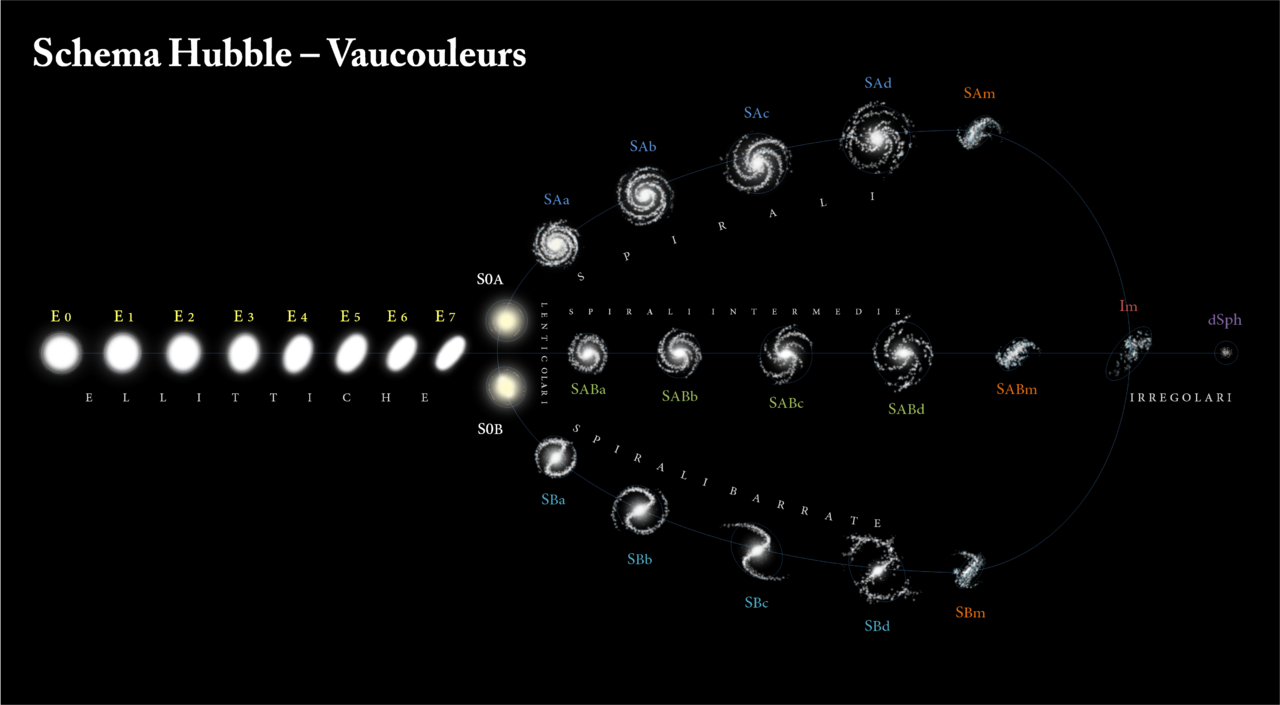
\includegraphics[scale=0.6]{hubble_mod.png}
  \caption[Diagrama de Hubble]{Diagrama de bifurcación mostrando la clasificación de Hubble con las modificaciones propuestas por De Vaucouleurs.}
  \label{tuningfork}
\end{figure}

\bigskip

\noindent Para las galaxias elípticas, el número $n$ después de la $E$ describe la elipticidad de la imagen, $n = 10 \times (a - b) / a$,
donde $a$ y $b$ son los ejes mayor y menor, respectivamente. De Vaucouleurs  propuso que las clases $Sd$ y $SBd$
deberían ser incluidas a la derecha de la secuencia y que las galaxias irregulares deben ser mostrada aun más a la derecha \citep{devaucouleurs1961}. Hubble creía que el diagrama de bifurcación era una secuencia evolutiva, por lo que para las elípticas, todavía se utiliza el término que propuso,``galaxias de tipo temprano'', mientras que para las espirales e irregulares les llamó consecuentemente, galaxias de tipo tardío. \footnote{ En este trabajo, se usará indistintamente estos términos por coherencia con la literatura, sin embargo, se debe recordar que solo son nombres históricos sin ninguna relación evolutiva.}


\bigskip

\noindent Las galaxias espirales están representadas en la ramas del diagrama bifurcación y se señalan con la letra $S$; las de la rama inferior son las  galaxias llamadas  espirales barradas, denotadas con el sigla $SB$. La letra minúscula después de la $S$ se basa en la apariencia de la estructura en espiral. $Sa$ y $SBa$ representa galaxias con brazos reforzados muy difusos y sus núcleos son grandes y luminosos. $Sb$ y $SBb$ caracterizan a las galaxias con brazos expandidos y pocos densos, con un pequeño bulbo. $Sc$ y $SBc$ son galaxias que tienen los brazos extendidos y pocos densos, con un bulbo aún menos brillante. Por último, las galaxias que marcan el punto de inflexión en el diagrama de bifurcación son las lenticulares y se denotan como $S0$. Estas galaxias se componen de un bulbo central y una estructura extendida en forma de disco que rodea a este bulbo. Las galaxias irregulares no tienen una estructura particular, se denotan con la sigla $Irr$ y la característica principal es que estas son asimétricas, sin bulbo central o sin espiral. En la clasificación ampliada, se colocan al final de la rama de las galaxias espirales.



\section{AGNs}

Dentro de ambos tipos (espirales ó elípticas) existen algunas que muestran un centro muy luminoso, del orden de $L \sim 10^{10} L_{\odot}$. A estas galaxias se les denominó como ``galaxias activas'' o actualmente como ``Núcleos Activos Galácticos'' (AGNs).
La característica principal que distingue a estos objetos de las galaxias inactivas (normales o regulares) es
la presencia de agujeros negros super-masivos que acretan materia en sus centros. Hasta la fecha, hay aproximadamente un millón de fuentes
conocidas de este tipo, seleccionado por su color y varios cientos de miles por espectroscopía \citep{santini2012}.

\bigskip

\noindent Se estima que en el Universo Local, a un \textsl{redshift} de $z \sim 0.1$, aproximadamente 1 de cada 50
galaxias contiene una hoyo negro super-masivo con rápida acreción, y aproximadamente 1 de cada 3
contiene uno de lenta acreción (\cite{richards2006}; \cite{rosario2012}). Los estudios detallados de grandes muestras de AGNs, la comprensión de su relación con las galaxias inactivas y su evolución con respecto al \textsl{redshift} comenzó a finales
1970, mucho después del descubrimiento de los primeros objetos cuasi-estelares (en lo sucesivo, cuásares) a principios de 1960.

\bigskip

\noindent  Debido a su importancia histórica, los primeros nombres que se les dieron a estos objetos, recuerdos de los años 60's y 70's, (e incluso más tarde) todavía se utilizan. Algunos de los nombres que aparecen ocasionalmente en la literatura, tales como ``Seyfert 1'' y ``Seyfert 2'', (en honor de Carl Seyfert, quien observó las primeras galaxias de este tipo
a finales de 1940), son el resultado de una de las primeras confusiones entre diferentes fuentes que ahora se sabe tienen propiedades similares. La principal diferencia observacional entre las \textsl{Seyfert} 1 y \textsl{Seyfert} 2 es su espectro  en el óptico-ultravioleta (UV).
Las \textsl{Seyfert} 1  muestran líneas permitidas muy fuertes y anchas ($\sigma$ $\sim$ 2000-10,000 km/s si se interpreta como ensanchamiento Doppler), mientras que las líneas en las \textsl{Seyfert} 2  tienen anchos que no exceden  $\sim$ 1200 km/s.

\bigskip

\noindent Tales diferencias ahora se entienden como el resultado de diferentes ángulos de visión a los centros de dichas fuentes y
también en parte, debido a una gran cantidad de oscurecimiento a lo largo de este. La nomenclatura común que se utilizará a lo largo de esta tesis es de AGN tipo I  para las fuentes que presenten una linea de visión despejada de sus centros y AGN tipo II para objetos afectados con oscurecimiento a lo largo la línea de visión que  extingue toda la radiación óptica-UV del interior. Las observaciones de los núcleos galácticos activos, (y otro ejemplo de clasificación) era la tendencia por separar el AGN según su luminosidad \citep{urry1995}. El nombre de ``galaxias Seyfert'' fue reservado para objetos de baja luminosidad, en su mayoría AGNs con bajo \textsl{redshift}, mientras que se llamó \textsl{QSO} a los miembros más luminosos de la familia. De hecho, la línea divisoria  entre galaxias \textsl{Seyfert} y cuásares no es muy precisa; algunos investigadores sugieren que la línea debe establecerse en alrededor de
$L_{bol}=10^{45}$ erg/s, donde $L_{bol}$ es la luminosidad  bolométrica de la fuente central \citep{antonucci1993}.

\bigskip

\noindent Otros prefieren una división basada en \textsl{redshift}, por ejemplo, en algunos trabajos todos los AGN con
$z \sim 0.2$ se consideran  cuasáres \citep{vanden2001}. Para añadir mas complejidad (o confusión), varios nombres se han propuesto en los últimos años para los AGNs con diferencias observacionales y propiedades físicas que  los originan: ``N-galaxias'', radio-galaxias de líneas anchas ``(BLRGs)'', radio-galaxias de línea angosta ``(NLRGs)'', galaxias en rayos
X con línea de emisión angosta``(NLXGs)'', objetos BL-Lac, QSO variable ópticamente violento ``(OVVs)'',
y  regiones de líneas de emisión de baja ionización nuclear  ``(LINERs)'' entre otros.
Para no entrar en confusiones, en este trabajo optaremos por utilizar el nombre genérico ``AGN''.

\bigskip

\noindent De este modo, podemos basar nuestra  definición de  actividad nuclear en galaxias
dada  por la huella observacional de esta actividad. Entonces, la definición
que usaremos es simple: un objeto extra-galáctico se considera que es un AGN sí
contiene una hoyo negro con acreción en su centro y sí se cumple al menos una de las siguientes características:

\begin{itemize}

\item Contiene una región nuclear compacta con emisión significativa, más allá de lo
se espera de los procesos estelares típicos de este tipo de Galaxias.

\item Se muestra la huella clara de un proceso continuo no estelar en emisión en
su centro.

\item Su espectro contiene fuertes líneas de emisión con relaciones de líneas que son típicos de
excitación por radiación no estelar.

\item Variaciones de líneas de emisión y/o del continuo.
\end{itemize}




\section{Bimodalidad}

Una vez establecida la existencia de los AGNs y su relación con el núcleo activo en cualquier tipo morfológico de galaxia,
 ya sea espiral o elíptica, regresamos  al tema de la morfología, la diferencia más notable en galaxias,visualmente hablando.
Las galaxias de diferente morfología presentan propiedades claramente diferenciadas, como en color (azul vs. rojo), en cinemática (soportado por presión o rotación), en luminosidad típica (menores vs. superiores),
en la agrupación con otras galaxias (menores vs. mayores entornos de densidad), etc. Muchas de estas diferencias son el resultado ó
se cree están relacionadas con las variaciones en el contenido de gas frío, que a su vez conducen a niveles diferentes de formación estelar. Las galaxias de tipo temprano, que incluyen elípticas y lenticulares ($S0$), fueron consideradas tradicionalmente como representantes de una población inactiva y son llamadas algunas veces como ``galaxias pasivas'' \footnote{También Conocidas equivalentemente en la literatura como \textsl{Quiescentes}}. La historia de formación de estas galaxias y otras de diferentes morfología, sigue siendo una de las cuestiones centrales en la investigación actual  \citep{perez2013} ;({\color{red} Ibarra-Medel, et.al. Submitted }).

\bigskip

\noindent Un salto importante para entender las diferencias en las propiedades de las galaxias debido a su morfología, se produjo con la llegada  del llamado  \textsl{Sloan Digital Sky Survey} (SDSS), \citep{york2000}. Con su gran muestreo espectroscópico de galaxias en el Universo Local, ($z \sim 0.1$, \cite{strauss2002}) además de su fotometría óptica en cinco bandas; el SDSS permitió el análisis estadístico de estas poblaciones. De esta forma se logró clasificar a una gran cantidad de galaxias en un diagrama que llamamos de color-magnitud (CMD) y este corroboró que las galaxias de campo forman dos ``picos'' en la distribución de color en el óptico \cite{strateva2001}; \cite{baldry2004}. El pico estrecho rojo ya había sido estudiada previamente en cúmulos de galaxias y era conocido como la \textsl{secuencia roja} \citep{devaucouleurs1961}.

\bigskip

\noindent El SDSS confirmó además que la secuencia roja, y en consecuencia las tempranas que se encuentran en ella, son abundantes en
ambientes aislados \citep{butcher1984}. El pico más amplio en la banda azul del óptico
se nombró como la nube azul. Las diferencias físicas entre las dos poblaciones
se exploraron a fondo y se cuantificaron por \cite{kauffmann2003}, quien encontró que las
galaxias en la secuencia roja tienen, en promedio, las poblaciones estelares de mayor edad,
mayor densidad de masa estelar superficial, y dominan a masas estelares mayores a $ \sim 10^{10.5} M_{\odot}$.


\bigskip

\noindent Esta bimodalidad de las distribuciones de color se convirtió no solo en un punto central en los estudios de galaxias locales, sino también con \textsl{redshifts}  mayores. \cite{bell2004} y \cite{faber2007} reportaron que la función de luminosidad de las galaxias de la secuencia roja se ha incrementado en un factor de dos o más desde $z \sim 1$. Este resultado sugiere que la acumulación de masa de las galaxias en la secuencia roja (y así posiblemente de galaxias tempranas) es un proceso que está en curso ($\sim$ 8 Gyrs). Este escenario estaría en desacuerdo con la imagen tradicional en el que las tempranas (especialmente elípticas) se formaron
en épocas muy tempranas en la historia del universo (es decir, deteniendo su formación estelar y convirtiéndose en galaxias de color rojo).

\bigskip


\noindent Esta imagen tradicional, tiene sus raíces en el escenario de colapso monolítico propuesto por \cite{eggen1962}, que posteriormente fue sustituido por el escenario jerárquico (por ejemplo \cite{kaufmann2006}) en el que las fusiones de las galaxias de disco proporcionan un mecanismo natural de formación de las galaxias elípticas \citep{barnes1996}. Si las fusiones siguen siendo importantes en las últimas épocas del universo, como algunas simulaciones numéricas sugieren, entonces se abriría la puerta para la formación tardía de galaxias elípticas y explicaría el crecimiento reportado de la secuencia roja.

\bigskip

\noindent Además, si las galaxias tempranas se continúan formando hasta épocas cosmológicas recientes, entonces  deberían existir galaxias que se encuentren actualmente en un proceso de transformación. Este tipo de galaxias tienen (o deberían tener) propiedades que estén entre las galaxias tardías y las galaxias de tipo temprano. Por ejemplo, deben tener algo de formación estelar, pero la mayor parte de la actividad debería haber cesado, es decir, la tasa de formación estelar ($SFR$), debería sería menor que el de las galaxias de tipo tardío de la misma masa. Por lo tanto, ¿cómo  puede identificarse tal población transitoria a gran escala?

\subsection{El Valle Verde}

Podemos definir al Valle verde como una región amplia y relativamente plana
(por lo tanto, `` valle") en el diagrama color-magnitud de galaxias,
que se encuentra entre los picos formados por  galaxias con formación estelar (nube azul)
 y las galaxias pasivas (secuencia roja). Además el valle verde
se ha propuesto  como el cruce en la evolución de las galaxias. Los
objetos en el valle verde se cree que representan la transición entre la nube azul de las galaxias de formación estelar y la
secuencia roja. ( \cite{kauffmann2003};\cite{wyder2007} ;\cite{schiminovich2007}; \cite{martin2007}; \cite{faber2007}; \cite{mendez2011}; \cite{goncalves2012}). En términos generales, se cree que todas las galaxias  siguen
trayectorias evolutivas similares en todo el valle verde, con una
rápida transición que explica la escasez relativa de las galaxias en el
valle verde en comparación con la nube azul o la secuencia roja \citep{haines2015}.

\bigskip

\noindent Los colores intermedios en el valle verde se
han interpretado como evidencia del apagado reciente de la formación de estrellas
\citep{salim2007}. La agrupación de
AGNs y sus galaxias huésped en el valle verde sugieren un papel más
para la retroalimentación del AGN en particular (por ejemplo,\cite{nandra2007}; \cite{hasinger2007}; \cite{silverman2008}; \cite{sanchez2004} ). Además, las galaxias en el valle verde tienen tasas de formación estelar (SFR) más bajas que la ``secuencia principal''
de formación de estrellas \citep{cano2016}, que es una correlación estrecha entre
la masa estelar y la tasa de formación de estrellas, posiblemente como resultado
de un apagado en la formación estelar  rápido (por ejemplo \cite{brinchmann2004}; \cite{elbaz2007};
\cite{salim2007}; \cite{noeske2007}; \cite{peng2010}).La mayoría de las galaxias de formación estelar
viven en la secuencia principal, por lo que el seguimiento de las poblaciones que salen de la
secuencia principal  (aquellos con bajos SFRs) se pueden utilizar para buscar el mecanismo de apagado en las mismas.

\section{Bimodalidad y Apagado en la Formación Estelar}

Hasta antes de la llegada de catálogos de galaxias espacialmente resueltas, la relación entre los mecanismos para la formación estelar y su apagado en galaxias se comprendía menos que hasta la fecha. Desde la perspectiva teórica, varios mecanismos de apagado en la formación estelar se propusieron, incluyendo por ejemplo:  el núcleo activo (AGN) y su retroalimentación (\cite{croton2006}; \cite{Hopkins2006}), \textsl{Shock Heating} en el halo (\cite{dekel2006}; \cite{cattaneo2006}), apagado  morfológico (\cite{martig2009}) y efectos de medio ambiente (\cite{gunn1972}; \cite{toomre1972}; \cite{moore1996}; \cite{bosselli2006}; \cite{weinmann2009}). Sin embargo, observacionalmente era extremadamente difícil identificar el mecanismo dominante. Por ejemplo, las galaxias masivas ($\sim$ $10^{11} M_{\odot}$ ) están preferentemente en regiones densas, es decir, efectos ambientales y por consiguiente el enfriamiento del halo podrían tener relación con estos procesos.

\bigskip


\noindent Para el caso de procesos internos, \citep{bluck2014} encuentran que el color (U-B) de una galaxia esta fuertemente ligada a una densa estructura interna y muestran además que la fracción inactiva está más estrechamente vinculada al bulbo. Dado la estrecha correlación entre la masa del bulbo y la masa del agujero negro, los autores sugirieron que la retroalimentación por AGN está más favorecida. Además, se sabe que muchas galaxias tienen una alta probabilidad de tener al mismo tiempo un bulbo con  AGN (\cite{kaufmann2006}; \cite{heckman2004}; \cite{schawinski2014}), lo que hace difícil aislar el efecto de una retroalimentación del AGN del bulbo central. Estas complejidades han obstaculizado en gran medida nuestro conocimiento del origen del apagado interno en formación estelar.

\section{El AGN como regulador de la formación estelar}

\noindent Una forma útil para seguir la evolución de galaxias observacionalmente es construir una función de luminosidad de todas las galaxias en un determinado \textsl{redshift}. La función de luminosidad $\Phi(L, z)$, se define de tal manera que $dN=\Phi(L, z) dVdL$ es el número de  galaxias por unidad de volumen co-movil, $dV$ a redshift $z$ en el intervalo de luminosidad
$L$, $L + dL$. El uso del volumen co-móvil, que se obtiene de la integración
del volumen entre $r(z)$ y $r(z + \Delta z)$ utilizando la cosmología supuesta, permite
una comparación directa de la misma población  en todos los \textsl{redshifts}.
Por lo tanto, $\Phi(L, z)$ proporciona una forma concisa para describir la evolución de galaxias en diferentes
tiempos cosmológicos \citep{kennicutt1998}.

\bigskip

\noindent Las luminosidades dependientes del \textsl{redshift} pueden ser comparadas con las predicciones teóricas que incluyen
solo enfriamiento bariónico simple. Dicha comparación muestra un ajuste entre el modelo y las observaciones para una amplia
gama de luminosidades alrededor de la $L_{*}$ . Sin embargo, el número calculado de galaxias más masivas ($\sim$ $10^{11}$ $M_{\odot}$) y las galaxias menos masivas ($\sim$ $10^{8}$ $M_{\odot}$) se desvían de las observaciones.
Por otra parte, hay una discrepancia significativa entre la predicción del enfriamiento atómico ya que debe llevar a la condensación
de alrededor del 80 por ciento de todos los
bariones \footnote{De vez en cuando usaremos la frase masa bariónica para referirnos a las simulaciones,
mientras que masa estelar define a las observaciones}
disponibles en gas y las estrellas en las galaxias. Sin embargo,las observaciones muestran que
esta fracción es inferior a 10 por ciento en $z = 0$.

\bigskip

\noindent Una posible solución es invocar un proceso de retroalimentación, es decir, un mecanismo que
inhiba el enfriamiento de gas y formación de estrellas en fases avanzadas de la formación de galaxias. Esto puede ser debido
a las estrellas ("retroalimentación estelar") o al AGN. Por
ejemplo, se piensa que en retroalimentación estelar la foto-ionización de
el gas bariónico en el halo puede retrasar la formación de galaxias pequeñas
en halos de materia oscura, lo que explica la falta de objetos en el extremo más bajo en la función de luminosidad.
Esto sin embargo, no puede explicar la falta de galaxias masivas $\sim 10^{11} M_{\odot}$ predichas por los modelos y otros procesos
de retroalimentación deben ser incluidos.


\bigskip

\noindent Como se mencionó, la correlación significativa entre la masa estelar (bulbo) y la masa del hoyo negro
en galaxias cercanas sugiere que la evolución del hoyo negro y la evolución de las galaxias van de la mano.
Esto plantea preguntas acerca la naturaleza de los procesos físicos que los enlazan, en particular, lo relacionado a que proceso
puede activar el hoyo negro central super-masivo  y apagar la formación estelar  en la galaxia huésped. Tal
proceso, si es lo suficientemente eficiente, pueden explicar la discrepancia entre las observaciones
con los cálculos de la función de luminosidad (en particular, la falta de grandes galaxias elípticas)
en comparación con las predicciones teóricas.

\bigskip

\noindent Esta retroalimentación se supone que puede venir en dos modos diferentes en épocas diferentes
durante el tiempo cósmico. En una fase temprana (a alto \textsl{redshift}) el
AGN puede apagar la formación de estrellas en las galaxias masivas. Es llamado el ``modo cuásar''
(\citet{croton2006}) y es más probable que venga acompañada de  un vigoroso
crecimiento lo que lleva a una fuerte retroalimentación cinética del agujero negro.
La otra forma de retroalimentación puede ser el AGN en ``modo regulador''. Este modo apaga la formación estelar en  épocas cosmológicas  recientes de tal manera que impide episodios significantes  de formación de estrellas \citep{fabian2006}. El acoplamiento entre la
acreción del agujero negro y el calentamiento  del gas esta limitados por lo dictado por las
observaciones .Sin Embargo, Si bien este tipo de hipótesis tienen éxito para subsanar algunas cuestiones clave, su principal problema es que la física de este proceso aún es poco conocido.

\section{Espirales Rojas: La Excepción a la Regla}

Como sucede en muchas ocasiones, existen excepciones a la regla y que nos obligan a cambiar el paradigma,
ya que se encontraron galaxias tardías o espirales con colores predominantemente rojos hace ya algún tiempo
(Por Ejemplo, \cite{bergh1976} sobre galaxias anémicas). El tamaño de su muestra era pequeño, sin embargo, quedo claro
que esos sistemas eran raros en el Universo Local. Esto implicaba que los procesos que llevaban a esos
objetos a ser rojos debían o ser raros, o producirlos solo por periodos cortos.
Cualquiera que fuera el motivo, estas espirales rojas eran  buenos laboratorios para estudiar
la evolución galáctica y comprender mejor como se ensamblaron las galaxias tempranas para formar la secuencia roja.

\bigskip

\noindent Otro de los proyectos interesantes que permitió una mejor comprensión de este grupo de galaxias es el famoso
\textbf{Galaxy Zoo}  (\cite{lintott2008})  que permitió distinguir una población significativa de espirales rojas (\cite{bamford2008}).
dentro de una selección de todas las galaxias espirales en general. Estos trabajos sugirieron que alrededor de 20 \% de esas galaxias se encuentran en la secuencia roja (y con una fracción creciente en regiones de densidad Media).
La fracción de espirales rojas parecía crecer con el medio ambiente, aún a masa estelar fija, implicando que algún proceso externo suprimía la formación de estrellas en las espirales rojas, mas allá de un simple cambio en la función de masa. (\cite{bamford2008})

\bigskip

\noindent Al mismo tiempo \citep{wolf2009} identificaron una muestra de espirales rojas y demostraron que estas tienen una tasa
de formación estelar (SFR) si bien baja, no era cero cuando se comparaba con las espirales azules.
Sin embargo, estos trabajos incluían espirales inclinadas. Esto como se sabe, puede hacer que galaxias azules se encuentren en la
secuencia roja debido a los efectos de enrojecimiento por polvo que depende de la inclinación (\citep{maller2009}, \citep{masters2010}).
También es bien sabido que las espirales con grandes bulbos pueden ser bastante rojas. Por ejemplo \citep{masters2010}
demostraron que esta tendencia en color debido al incremento en el bulbo es comparable en tamaño al enrojecimiento por inclinación.
Por esa razón \citep{masters2010} seleccionaron una nueva muestra de espirales de cara del \textsl{Galactic Zoo} con bulbos pequeños para
estudiar las propiedades  de espirales intrínsecamente rojas.
De esas espirales de cara, encontraron que alrededor del 6\% caen en la secuencia roja
(incrementando en 30\% cuando se incluían galaxias dominadas por bulbo). Además mostraron que sí bien tienen una tasa de formación estelar baja, no son objetos completamente pasivos (lo cual confirmó \cite{cortese2012}). La fracción de galaxias tardías en la secuencia roja se incrementaba sustancialmente con la masa estelar, pero a toda las masas estelares la población de espirales rojas parecían tener una población estelar más vieja y una menor formación estelar reciente que las espirales azules.

\bigskip

\noindent Mientras que las tardías rojas son relativamente raras en el Universo Local, estas podrían formar un camino importante para entender la evolución entre la nube azul y la secuencia roja. \citep{bundy2010} uso datos del COSMOS \textsl{survey} \citep{cosmos2007} para estudiar la secuencia roja de galaxias con morfología de disco a altos \textsl{redshifts} y concluyó que una cantidad significativa de galaxias con disco se traslada de la nube azul a la secuencia roja (60\%) pasando por una fase de espiral roja. \citep{robaina2012} comparó la población estelar de una muestra de galaxias con morfología espiral o elíptica y que fueron seleccionadas por su pasividad y su bajo enrojecimiento por polvo. Estas espirales rojas por definición, eran más pasivas que la muestra de \citep{masters2010} y además no hizo ninguna selección por el tamaño del bulbo. El trabajo de \citep{robaina2012} encontró que la población estelar en las dos muestras (en edad y metalicidad) eran estadísticamente indistinguibles.

 \section{UGC11680}

 La galaxia espiral UG11680 pertenece al tipo de galaxias tardías que se menciona en la sección anterior. Su color rojo podría ser
 indicador de que ha dejado de formar estrellas y aún conservar su morfología espiral, por lo que puede ser un laboratorio para analizar
 el proceso que llevo a ese color.

 \begin{figure}[!ht]
   \centering
   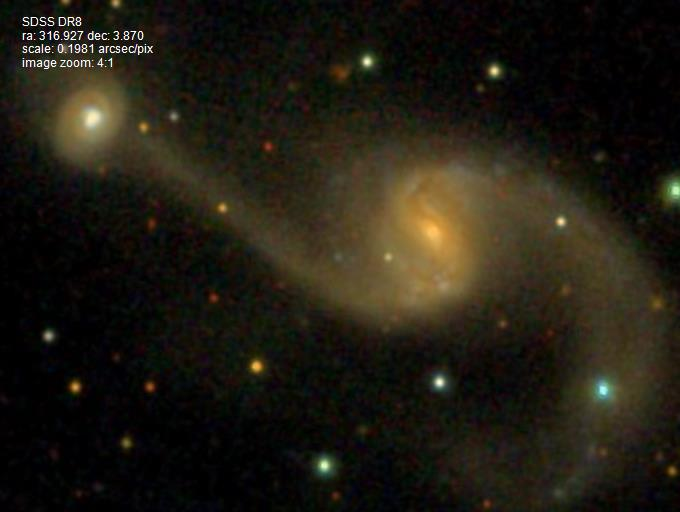
\includegraphics[width=4in]{ugc11680.jpg}
   \caption[ Imagen de UGC11680]
    {Imagen en el óptico de UGC11680 (SDSS8).}
 \label{ugc11680}
 \end{figure}


 \noindent UGC11680 es una espiral SBb con AGN tipo 2, con un color rojo en el óptico, lo que la ubica en la secuencia roja del diagrama color magnitud. Los valores que utilizaremos se encuentran recopilados en la tabla \ref{tab_valores}. Si se requieren otros datos, se darán dentro del texto mismo. Haciendo una búsqueda rápida en la literatura se menciona en 17 artículos hasta la fecha.
 Es incluida por primera vez en \citet{hewitt1991} el cual es un catalogo de objetos cuasi-estelares.
 En los años siguientes, es incluida en diferentes estudios de galaxias \textsl{Seyfert} así
 como catálogos de ellas, por ejemplo \citep{thean2000}; \citep{klimanov2001}; \citep{tran2003}. Es interesante notar el artículo  \citet{moustakas2006}  ya la incluye en el grupo de galaxias peculiares. Prosiguen más estudios sobre poblaciones de galaxias \textsl{Seyfert} hasta que se menciona en la presentación del survey \textbf{CALIFA} \citep{sanchez2012}. Dentro de los artículos de la colaboración de \textbf{CALIFA} se menciona en tres: en estudios de galaxias LINERs \footnote{tipo de galaxia que tiene una emisión nuclear de baja ionización. Esta en debate actual si se considera esta ionización un producto del AGN o simplemente de la emisión de estrellas post-AGB} \citep{singh2013}, en estudios de cinemática de gas en galaxias en proceso de fusión \citep{barrera2015} y su clasificación como barrada para estudiar esta propiedad \citep{blazquez2007}, aunque en el catálogo de NED  UGC11680 está clasificada como Scd, mantendremos la morfología barrada. Una imagen de UGC11680 obtenida de SDSS 8 se muestra en la Figura \ref{ugc11680}.

 \begin{table}[!ht]
 \centering
 \begin{tabular}{||c | c||}
 \hline
 \hline
 Valores Principales & UGC11680NED01 \\
 \hline
 \hline
 Centroide & 36.840,31.753 \\
 Redshift & 0.025887\\
 $R_e$ (kpc) & 8.189 \\
 Log Masa St sin corregir  & 11.337\\
 $H_{\alpha}/H_{\beta}$ & 4.052 \\
 Promedio $A_v$ & 1.092  (mag) \\
 $A_v$ ponderado  & 1.674  (mag) \\
 SFR & 4.143 ($M_{\odot}/yr^2$) \\
 log SFR & 0.617 $\log_{10}$ $(M_{\odot}/yr^2)$ \\
 Ionización Central & sAGN  $>$ Kewley y $|EW (H_{\alpha})|>6$\\
 Velocidad Sist Gas & 7771.840 km/s \\
 Velocidad sistemica SSP & 7749.618 km/s \\
 \hline
 \hline
 \end{tabular}
 \caption[Datos de UGC11680] {Valores Principales UGC11680 (obtenidos de aplicar \textbf{PIPE3D} al cubo de datos de UGC11680)}
 \label{tab_valores}                              %etiqueta para referencia
 \end{table}




%%%%%%%%%%%%%%%%%%%%%%%%%%%%%%%%%%%%%%%%%%%%%%%%%%%%%%%%%%%%%%%%%%%%%%%%%
%                           Objetivo                                    %
%%%%%%%%%%%%%%%%%%%%%%%%%%%%%%%%%%%%%%%%%%%%%%%%%%%%%%%%%%%%%%%%%%%%%%%%%

\section{Objetivos}
En este trabajo nos concentraremos en un solo aspecto para estudiar a la galaxia UGC11680: sus poblaciones estelares  y por lo tanto la información que requerimos para empezar a comprender por que tiene este color rojo.

\bigskip

\noindent Aunque es solo una galaxia, los resultados de su estudio  nos darán pistas para continuar resolviendo y tratando de entender la evolución galáctica y ofrecer un método sólido para su estudio. Por ejemplo, con imágenes multi-banda con buena resolución espacial, es posible resolver la historia de formación estelar en espacio y tiempo, lo que ya ha sido hecho con anterioridad (por ejemplo, \citet{brinchmann2000}; \citet{kong2000}; \citet{perezg2008}) y el llamado método de registro fósil ha sido
ampliamente utilizado para recuperar las historias de formación estelares
utilizando  datos espectrales y fotométricos (\citet{kaufmann2006}; \citet{cid2005}; \citet{gallazzi2005}).
Por otro lado, estos estudios están limitados por el tamaño de la apertura (para el caso de los datos de espectroscopía).
La resolución espectral (en el caso de imágenes multi-banda) pueden generar un sesgo importante en la interpretación de los datos y por consiguiente las conclusiones sobre los procesos evolutivos.

\bigskip

\noindent Es interesante notar que una apertura con tamaño fijo no puede resolver localmente las propiedades de las galaxias debido a que el espectro de la galaxia observada integra toda o una fracción sustancial de la luz dentro de una apertura. Para el caso de los estudios fotométricos, se requiere un número de bandas fotométricas lo suficientemente grandes como para
producir el espectro de galaxias. Sin embargo, con la llegada de la espectroscopía 3D o espectroscopia de campo integral (IFS),  es
posible acceder a los datos espectrales resueltos para diferentes
regiones de galaxias y obtener así espectros locales (por ejemplo, \cite{cappellari2012}; \cite{croom2012}; \cite{sanchez2012}; \cite{cid2013_1}; \cite{bundy2015} ).

\bigskip


\noindent Con datos IFUs y  la descomposición con poblaciones estelares simples (SSP), es factible no sólo
obtener información de como UGC11680 ensambló su  masa estelar, sino también es posible entender la forma en que esta se ensambló a nivel local. Trabajos observacionales recientes indican que una fracción importante
de las galaxias estudiadas tienden a formar la mayor parte de sus masas estelares en su parte interna más rápido que en su exterior,
lo que sugiere que estas galaxias ensamblan sus masas
desde dentro hacia afuera ( \citet{blazquez2007}; \cite{perez2013}) ({\color{red} Ibarra-Medel, et.al. Submitted }).

\bigskip

\noindent Por ejemplo, usando datos de \textbf{CALIFA} \cite{perez2013} mostraron que la velocidad de este proceso
depende de la masa total de la galaxia estelar. Además, hay indicios de
una fase de transición en la que se cambia el crecimiento de masa de las galaxias de dentro hacia afuera
a un gradiente de afuera hacia adentro y que depende de la masa de las galaxias (\cite{perez2013}). Así, es fundamental la comprensión de cómo algunas galaxias apagan su formación de estrellas, lo que regula su crecimiento. Este apagado
se denomina comúnmente en la literatura  como``quenching'', y
podría ser utilizado para explicar la formación y consecuente declinación en formación estelar en UGC11680 durante su evolución.

\bigskip

\noindent Aunque solo se trata de una galaxia, el estudio y manejo comparativo de las historias de formación estelar
son novedosas y no encontradas hasta la fecha en la literatura. Por lo tanto,
en análisis futuros se podría utilizar este método para una muestra mas significativa de galaxias.
Al poder utilizar métodos que nos permiten observar las épocas de formación galáctica, daremos un paso adelante para contribuir
en el análisis y posiblemente utilizarlo en diferentes variables de interés.

\bigskip


\subsection{Estructura de la tesis}

Este trabajo está dividido en 3 Capítulos y un apéndice, y se explican como sigue:

\begin{itemize}

\item El primer capítulo incluye la introducción, donde incluimos los antecedentes generales del estudio de objetos extra-galactico, la definición de AGN y sus propiedades esenciales; una breve discusión sobre la bimodalidad y el estado del arte como diagrama evolutivo. Presentamos además a la galaxia UGC11680 y sus características principales.


\item En el siguiente capitulo se explicará brevemente el muestreo de \textbf{CALIFA}, que son los IFUs y el proceso de análisis de los cubos y los datos que se obtengan de ellos. Después haremos un chequeo general del enrojecimiento  por polvo y analizaremos la tasa de formación estelar de UGC11680 con respecto a las galaxias de la muestra. Una vez descartado el enrojecimiento por polvo, explicaremos el proceso para obtener las poblaciones estelares y que servirán para obtener el producto final, la historia de formación estelar con su mapa $SFH(t,R)$; Esto es importante, ya que todo nuestro análisis posterior depende de este parámetro.

\item El capítulo final incluirá el análisis sobre la historia de formación estelar espacialmente resuelta para la galaxia UGC11680 y para diferentes tipos de galaxias, promediadas en diferentes categorías. Se compararán estas historias en base al parámetro  $\chi^2$ y esto nos indicará a que promedios se parece ó ajusta más UGC11680 con respecto a su historia de formación estelar.

\item Finalmente incluimos un breve apéndice en donde se incluye por que sabemos que UGC11680 es una galaxia con AGN.

\end{itemize}

\noindent La galaxia de estudio UGC11680 se dividió en 3 zonas de estudio determinadas por su radio efectivo. A lo largo de esta tesis, llamamos ``partes centrales'' a la zona comprendida por $0< R/R_e < 0.5$, ``partes medias'' a la zona $ 0.5< R/R_e < 1.25 $ y las zonas externas o las ``afueras'' a $1.25<R/R_e < 2.0$.

\bigskip

\noindent Finalmente, en este trabajo los parámetros cosmológicos utilizados fueron $\Omega_m = 0.317$ , $\Omega_{\Lambda}=0.683$ y $H_0 = 67.15$ km/s/Mpc \citep{plank2014}

            % ~10 páginas - Explicar el propósito de la tesis
%
%%%%%%%%%%%%%%%%%%%%%%%%%%%%%%%%%%%%%%%%%%%%%%%%%%%%%%%%%%%%%%%%%%%%%%%%%
%           Capítulo 2: MARCO TEÓRICO - REVISIÓN DE LITERATURA
%%%%%%%%%%%%%%%%%%%%%%%%%%%%%%%%%%%%%%%%%%%%%%%%%%%%%%%%%%%%%%%%%%%%%%%%%

\chapter{Marco teórico}
En este capítulo, normalmete se ponen todas las ecuaciones que se van a usar en la tesis, así ya nomás se hace rferencia a la ecuación tal o "como se vió en el capítulo 2", y esas cosas.
%inserción de codigo de Matlab
%Es conveniente sangrarlo (los de proteco dicen "indentarlo") para que no se encime con los números  de las líneas a la izquierda
\begin{lstlisting}[frame=single]
    % Declaracion de las variables simbolicas
    syms u z1 z2 z3 z4 J m M g l 
    % Matrices involucradas
    E = [J+m*l*l m*l*cos(z1);m*l*cos(z1) M+m] 
    F = [m*g*l*sin(z1);u+m*l*(z3*z3)*sin(z1)] 
    % Despeje
    V = E\F
\end{lstlisting}

\blindtext           % ~20 páginas - Poner un contexto a la tesis, hacer referencia a trabajos actuales en el tema

%%%%%%%%%%%%%%%%%%%%%%%%%%%%%%%%%%%%%%%%%%%%%%%%%%%%%%%%%%%%%%%%%%%%%%%%%
%           Capítulo 3: NOMBRE                   %
%%%%%%%%%%%%%%%%%%%%%%%%%%%%%%%%%%%%%%%%%%%%%%%%%%%%%%%%%%%%%%%%%%%%%%%%%

\chapter{Estudio de las poblaciones estelares}

\lettrine[lines=1]{E}n este capitulo analizaremos las poblaciones estelares de UGC11680 y así mismo estudiaremos el enrojecimiento por polvo y la tasa de formación estelar.

\section{Espectroscopía De Campo integral}

La espectroscopía de Campo Integral (de aquí en delante IFS por sus siglas en
inglés, \textit{Integral Field Spectroscopy}) es una técnica de observación astronómica capaz de obtener simultáneamente y en una sola
exposición espectros de típicamente muchos elementos espaciales (\textit{spaxels}) de una fuente sobre un campo de visión bidimensional.
Un espectrógrafo de campo integral consiste de dos componentes: el espectrógrafo y la unidad de campo integral (IFU por sus siglas en inglés, \textit{Integral Field Unit}) cuya función es dividir el plano espacial 2D en un arreglo de \textit{spaxels}
individuales y dirigir el haz de luz de cada uno de ellos al espectrógrafo, de manera que obtenemos una gran cantidad de imágenes
cada una a diferente longitud de onda. En general, todas ellas pueden formar un cubo de datos con la información
en tres dimensiones, dos espaciales $X$, $Y$ (declinación y ascensión recta) y longitud de onda. Ver Figura \ref{cubo}


\begin{figure}
  \centering
    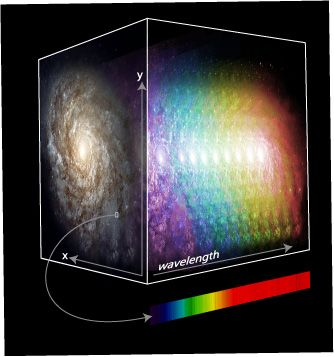
\includegraphics[scale=0.5]{data-cube-illustration.jpg}
  \caption[Cubo de Datos]{Representación esquemática de un cubo de datos.}
  \label{cubo}
\end{figure}

\subsection{CALIFA}

El \textit{Calar Alto Legacy Integral Field Area Survey} (\textbf{CALIFA}) \citep{sanchez2012}
fue un  proyecto  del Centro Astronómico Hispano-Alemán en el Observatorio de Calar Alto para
obtener espectros espacialmente resueltos de 600 galaxias del Universo Local ($0.005 <z <0.03$)
por medio de espectroscopía de campo integral (IFS). Las observaciones en \textbf{CALIFA}
comenzaron en junio de 2010 con el espectrografo Multi-Apertura Postdam (PMAS), montado en un telescopio de 3-5m,
utilizando  campo de visión hexagonal (FOV) \citep{Verheijen2004}.

\bigskip

\noindent En este espectrógrafo, se observó cada galaxia usando dos configuraciones diferentes,
una resolución del intermedio espectral (V 1200, R $\sim$ 1650) que cubre la gama del azul en el óptico (3700-4700 \text{\AA})
y una de baja resolución  (V 500, R$\sim$ 850) que cubre el primer orden de la longitud de onda óptica (3750-7500 \text{\AA}.
(Para este trabajo se utilizó los cubos de datos del V500).

\bigskip


\noindent Una muestra seleccionada  de 939 galaxias se extrajo de la séptima publicación de los datos del SDSS,
que es se describe en \citep{walcher2014}. A partir de esta muestra, 600 galaxias son seleccionadas al azar.
La combinación de técnicas de imagen y espectroscopía óptica a través de IFS proporciona una visión más completa de propiedades
de las galaxias individuales que cualquier survey tradicional y en comparación con otros surveys IFS, \textbf{CALIFA} ofrece para nuestro caso las siguientes características:


\begin{itemize}

\item Una muestra que abarca una amplia gama de tipos morfológicos, cubriendo toda la secuencia de Hubble , desde elípticas (E0-E7), lenticulares (S0-S0a) a espirales, además de un amplio rango de masas ($10^9$ $\sim$ $10^{12}$ $M_{\odot}$)

\item Una muestra que cubre todo el  diagrama color-magnitud para $M_r > - 18$ mag que nos permite obtener relativamente bien las poblaciones galácticas (secuencia roja, nube azul y valle verde);

\item Observaciones que cubren el rango la longitud de onda  del espectro óptico, que nos permite obtener la historia de formación estelar para las poblaciones estelares subyacentes.

\end{itemize}

\noindent En artículos previos con esta muestra, y usando las historias de formación estelar de $\sim$ 100 galaxias \citep{perez2013} derivaron la información espacialmente resuelta del crecimiento de masa galáctica. Además, \citep{gonzalez2014} describieron  las propiedades de las poblaciones estelares. Ambos artículos confirmaron que las galaxias masivas acumulan su masa estelar de dentro hacia afuera. Encontraron además que las galaxias más masivas eran más compactas, viejas, mas ricas en metales y menos enrojecidas por polvo.
De esta forma usaremos varios de estos métodos descritos en estos y otros trabajos con la muestra de \textbf{CALIFA}.

\subsection{Enrojecimiento por Polvo}

Antes de avanzar en el estudio de las poblaciones estelares de la galaxia UGC11680,
revisamos la atenuación por polvo en ella, ya que es posible
que solo sea este lo que la vuelve mas roja. Para cuantificar el nivel de
extinción en UGC11680 comparamos en su espectro integrado la diferencia en flujo en las primeras dos
linea de la secuencia de Balmer ($H\alpha$ y $H\beta$). La razón esperada entre los flujos de estas dos líneas
es de $R_{int}=F\alpha/F\beta=2.86$ \citep{osterbrock1989}. Por lo tanto, desviaciones de esa relación se pueden usar para medir
la extinción relativa entre $H\alpha$ (a 6562.8 \text{\AA} en la banda r) y $H\beta$ (a 4861 \text{\AA} en la banda g).

\begin{figure}
  \centering
    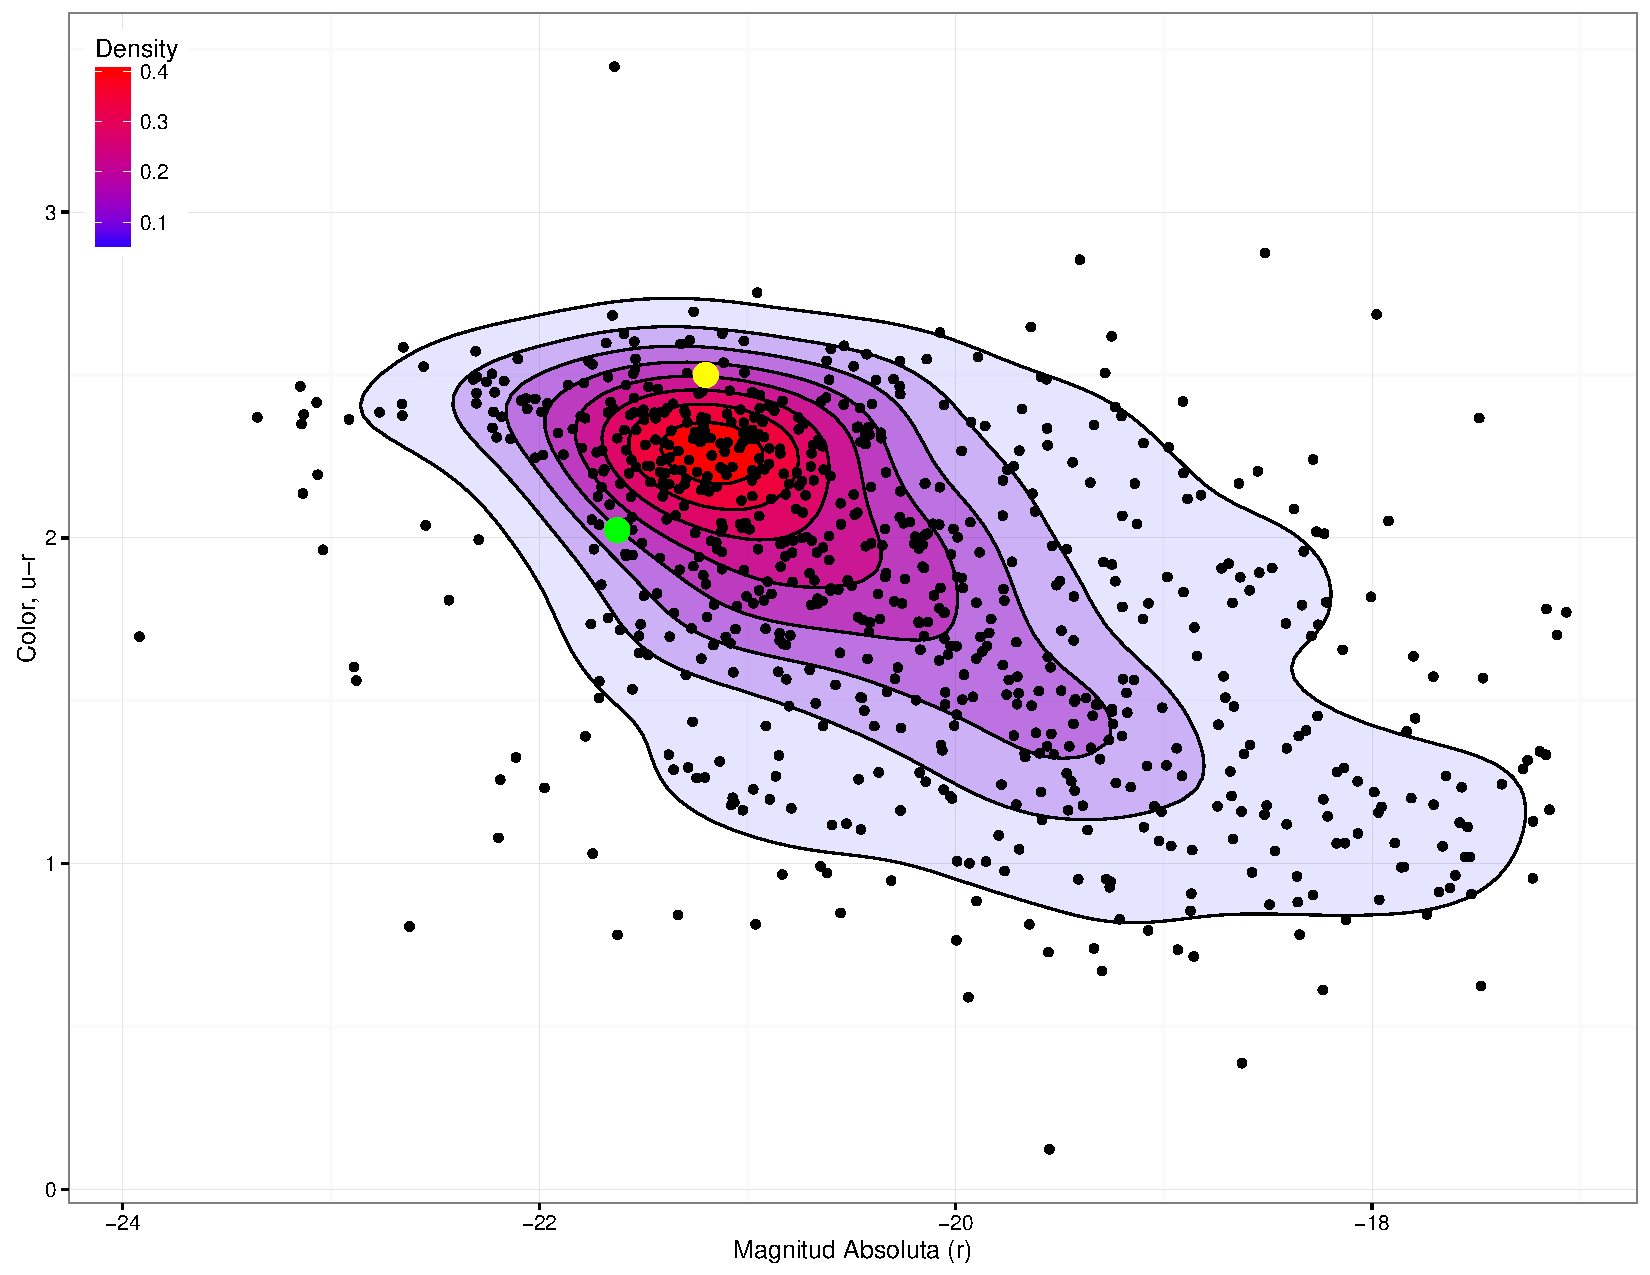
\includegraphics[scale=0.5]{color_magnitud_ur.pdf}
  \caption[Diagrama Color-Magnitud con UGC11680]{Diagrama en Color Magnitud para las galaxias de la muestra de  \textbf{CALIFA}. Marcamos las posiciones de la galaxia UGC11680 por dos puntos. El punto amarillo representa a UGC11680 sin corregir por polvo y el punto verde lo muestra ya corregido. Nótese que a pesar de que el polvo la enrojece, ese enrojecimiento no es suficiente para sacarla de la secuencia roja.}
  \label{cmd1}
\end{figure}


\noindent A raíz de la relación de extinción empírica, las luminosidades intrínsecas, $L _{int}$, están dadas por

\begin{equation}
L _{int} (\alpha) = L_{obs} (\lambda) 10^{0.4A_{\lambda}} =L_{obs} (\lambda) 10^{0.4k(\lambda)E(B-V)}
\end{equation}

\noindent donde $L_{obs}$ son las luminosidades (extinguidas) observadas, $A(\lambda)$ es la extinción a la longitud de onda $\lambda$,
 y $k(\lambda)$ de la curva de enrojecimiento.El exceso de color se define por

\begin{equation}
E(B -V) =(B - V)_{obs}-(B - V)_{int}
\end{equation}

\noindent que es el cambio en el  color $(B - V)$  debido al polvo (es decir, la diferencia entre el color observado y esperado
en ausencia de polvo). El decremento de Balmer intrínseco se mantiene constante para condiciones típicas de gas \citep{osterbrock1989}, por lo que


\begin{equation}
E(H\beta - H\alpha) = 2.5 \log \frac{F_{obs}}{F_{int}},
\end{equation}





\noindent y por lo tanto un calculó con los datos obtenidos del cubo de datos perteneciente a la galaxia UGC11680 que se muestran en
la tabla \ref{tab_valores} nos da finalmente una  $A_V \sim 1$ mag. El resultado se muestra con el diagrama de color magnitud de la Figura \ref{cmd1}. La posición de UGC11680 se muestra con puntos en el diagrama y su corrección también se muestra en este. El diagrama también muestra la secuencia roja  en nuestra muestra. Hay que notar que la galaxia UGC11680 perdió posición dentro de esta densidad corregida, sin embargo no es suficiente para que salga de la secuencia roja.


\bigskip


\noindent Esto nos da una idea de lo que esta pasando. En general, \citep{sanchez2012} para las galaxias de cara con morfología Sb-Scd, la extinción esta en el rango de $A_V \sim 1.3$ mag. Así, La galaxia UGC11680 tiene un valor relativamente normal de extinción para las galaxias de su tipo y se encuentra dentro de los rangos comunes para las galaxias de cara y no es suficiente para sacarla de la secuencia roja de la muestra y así lo indica la Figura \ref{cmd1}. Esto ya elimina la extinción como causante de que UGC11680 se encuentre en la secuencia roja.





\subsection{Tasa de formación estelar}

La tasa de formación estelar (SFR) es la masa de gas convertido en estrellas por unidad de tiempo.
La unidad estándar para medir el SFR es la masa solar por año ($M_{\odot}/ yr$). La SFR puede
medirse en pequeñas regiones de una  galaxia, como una nube molecular única, en
galaxias, y en todo el universo. La SFR a un \textsl{redshift} dado es un elemento esencial de
información sobre la evolución de una determinada galaxia o toda la población de ellas
en ese tiempo. Seguir la SFR en el tiempo es equivalente a seguir el ensamblaje de la masa estelar
en el universo. Hay varios métodos empíricos para estimar el SFR desde el ultravioleta, óptico,
y a partir de observaciones en el infrarrojo. Todos los métodos se basan en la teoría estándar de formación de estrellas
 y emplea diferentes tipos de emisión asociados a este tipo de eventos.

 \begin{figure}
  \centering
    \includegraphics[scale=0.5]{sfr_califa2.pdf}
  \caption[Diagrama de Tasa de Formación estelar]{Tasa de Formación estelar con respecto a
           la masa estelar para la muestra de \textbf{CALIFA} en escala logarítmica. En este diagrama La posición de la galaxia
          UGC11680 dentro del diagrama se marca con el punto azul. En este diagrama se observa lo reportado en \cite{cano2016}, la existencia de dos secuencias: la de las galaxias formadoras de estrellas y las retiradas. Nótese que la galaxia UGC11680 se encuentra debajo de la secuencia de galaxias formadoras de estrellas y sobre la secuencia de las retiradas. }
  \label{sfr_califa}
\end{figure}


\bigskip

\noindent En \citep{sanchez2013} se derivó la tasa de formación estelar sumando los flujos de $H \alpha$ de las regiones $HII$ dentro del campo de visión de las galaxias de la muestra de \textbf{CALIFA}, con atenuación por polvo usando una extinción promediada derivada de esas regiones. Aunque hay una discrepancia entre las tasas derivadas, aquí se asume una tasa de formación de \citep{kennicutt1998}


\begin{equation}
SFR(Myr^{-1})= 7.9 \times 10^{-42} L_{H_{\alpha}} (\text{erg} \text{s}^{-1})
\label{tasa}
\end{equation}



\noindent Para el caso de la galaxia UGC11680 la tasa de formación estelar estimada con esta relación resultó ser $\log$ $SFR$ $\sim$ 0.6 $\log_{10}$ $(M_{\odot}/yr^2)$ ó $SFR \sim $  4.1 ($M_{\odot}/yr^2$).

\subsection{La secuencia de galaxias formadoras de estrellas}

Una de las formas de visualizar la propiedades de evolución de las galaxias es graficar la SFR contra la masa estelar $M_{*}$
para todas las galaxias de la muestra. Tal diagrama se muestra en la Figura \ref{sfr_califa} y sobresalen dos cosas. Una, la secuencia que contiene a las las galaxias que forman estrellas. A las galaxias que están concentradas en esa secuencia a veces se le llama galaxias de secuencia principal ó galaxias SF; segundo, la secuencia debajo de la SF, que es conocida como de las galaxias retiradas o galaxias que en su mayoría dejaron de formar estrellas.

\bigskip

\noindent En \citep{cano2016} se reporta un valor de 0.81 en la pendiente de galaxias formadoras de estrellas en la muestra de \textbf{CALIFA}. Para nuestro caso y con los datos dados en la
introducción, encontramos un valor de $\beta=0.83$ donde $\beta$  es la pendiente de la relación. En ese mismo artículo
se encuentra que las galaxias retiradas tienen una pendiente de $\beta \sim 0.86$  por lo que coloca a UGC11680 en el
lugar entre las galaxias retiradas y las galaxias en la SF. Es interesante notar que  UGC11680 se encuentra entre estas dos secuencias en la Figura \ref{sfr_califa}. Esto implica que  UGC11680, deja de formar estrellas pero no completamente, lo que podría ser un indicador de que el AGN de UGC11680 es un tipo de regulador de formación estelar. Esta implicación podría tener consecuencias relevantes en el estudio que sigue.



\section{Análisis de poblaciones estelares}

La masa también es un factor fundamental en la evolución galáctica. Como se mencionó en la introducción, la mayor parte de las galaxias se han formado a través de fusiones e interacciones de forma jerárquica, es decir, pequeños sistemas se han fusionado para formar sistemas más grandes. A épocas cosmológicas tempranas, la formación estelar era más efectiva en galaxias masivas pero en épocas cosmológicas más recientes la formación estelar se apagó en galaxias masivas, pero continuó en galaxias más pequeñas ,un fenómeno llamado ahora ``downsizing'' \citep{corteau2014} ({\color{red} Ibarra-Medel, et al. Submitted }).

\bigskip

\noindent Así mismo, las galaxias brillan por que sus estrellas radian la energía que producen por reacciones nucleares en sus centros. La teoría de evolución estelar describe la cantidad de energía liberada  por una estrella dada su masa inicial. Entonces, modelando la luz emitida por todas sus estrellas en una galaxia sobre todas sus longitudes de onda se obtiene la llamada ``distribución de energía espectral'' (SED), y así se puede derivar (en principio) la masa estelar que es responsable de esa radiación. Históricamente, como había sido señalado por Baade \citep{baade1957}, nuestra propia Vía Láctea esta compuesta de varias poblaciones estelares, por lo que las galaxias en general se pueden descomponer en poblaciones estelares con propiedades comunes. Podemos definir entonces una población estelar simple (SSP) como un grupo de estrellas que evolucionan de la misma manera, con una misma composición química (al nacer) y cinemática similar.

\bigskip

\noindent Un ejemplo de estas SSP en la naturaleza, son los cúmulos globulares (abiertos o cerrados). La incertidumbre  en estas SSP sería la llamada función de masa inicial (IMF) que da el espectro de masa de la generación estelar al nacer. Esta no se deriva por primeros principios. Modelos  empíricos de esta IMF, basados en la vecindad solar fueron  descritos por primera vez por Salpeter, como una ley de potencia con un exponente de $\sim$ -2.35 \citep{salpeter1955}. Así, un IMF debe ser postulado cuando se calculan  las propiedades de esta poblaciones. Por lo tanto, el espectro de una galaxia puede ser en principio modelado por una combinación lineal de SSPs, esto es, $ Galaxia = \sum_{j} SSP_{j}$.

\bigskip

\noindent El propósito principal de ajustar el espectro de UGC11680 (ó cualquier otra galaxia de la muestra de \textbf{CALIFA}) con múltiples SSPs, es reconstruir su historia de formación estelar bajo el supuesto de que el continuo estelar es la suma de diferentes componentes, cada uno de ellos correspondientes a a un brote particular de formación estelar y así a una SSP particular con su propia edad y metalicidad. Sin embargo, en la práctica esto es un poco más complicado, ya que se deben incluir todos los SSPs que se elijan para esto, la atenuación por polvo (que puede ser diferente para cada SSP) y la cinemática estelar (velocidad sistémica y dispersión). Adicionalmente, se tienen las emisiones de gas ionizado que pueden afectar el resultado, ya que algunas líneas afectan las características indicativas de la edad. En \citep{pipe1} se presentan una serie de algoritmos para analizar espectros con poblaciones estelares más complejas, enfocado en los espectros de IFUs en el óptico. Estos algoritmos llamados en su conjunto como \textbf{Fit3d} y su pipeline llamado \textbf{Pipe3D} \citep{pipe2}. Con estas herramientas, realizamos el análisis de los cubos de datos de nuestra muestra. Los principales artículos en los que se basó esta descripción fueron \citep{pipe1} y \citep{pipe2}, que pueden ser consultados si se necesita una descripción más detallada.

\bigskip

\noindent Las SSPs utilizadas en este trabajo constan de una librería definida como \textbf{gsd156}. Esta librería se detalla
en \cite{cid2013_1}. Incluye 156 plantillas que cubren 39 edades estelares (desde 1 Myr a 14 Gyrs) y cuatro metalicidades
($Z/Z_{\odot}$= 0.2, 0.4, 1 y 1.5). Estas plantillas fueron extraídas de una combinación espectros estelares sintéticos
de \textbf{GRANADA} \citep{martins2005} y las librerías de SSPs del proyecto \textbf{MILES} (\cite{blazquez2006};\cite{vazdekis2010}; \cite{falcon2011}). Estas SSPs usan la función inicial de masa de Salpeter, mencionada anteriormente.

\bigskip

\noindent Finalmente, antes de describir el proceso de \textbf{Fit3D} damos las siguientes definiciones:

\begin{itemize}

\item Definimos un cubo de datos como un archivo 3D que comprende las 2 primeras dimensiones con a distribución espacial de pixeles $X,Y$ y la tercera dimensión con la información de la longitud de onda de los datos en el cubo ($Z$). Los cubos de datos almacenados, incluyen los datos con la misma distribución espacial en la dirección en $X$ y $Y$ (en arco-segundos) y la misma distribución en longitud de onda en la dirección-$Z$ (en \text{\AA})

\item Un archivo ``RSS'' (espectros apilados en renglones) como un archivo fits 2d que incluye espectros en $NY$ de la misma longitud $NX$ con longitud de onda normalizada. Este archivo esta normalmente relacionado con una tabla de posiciones que es un archivo ASCii con $NY$+1 renglones.

\item Finalmente, definimos ``mapa'' como un archivo fits de 2 dimensiones que comprende la distribución espacial de cierto parámetro.

\end{itemize}



\noindent En general, los espectros que tienen los cubos de datos de \textbf{CALIFA} tiene una señal a ruido $S/N$ arriba de 50 para la mayoría de las galaxias incluidas en el catálogo de IFUs de interés \citep{sanchez2012}. Sin embargo, conforme el brillo superficial declina como función de la distancia galactocéntrica, la $S/N$ decrece rápidamente en las regiones exteriores \citep{sanchez2012}. Para subsanar este problema se  propone un algoritmo basado tanto en un criterio de continuidad en el brillo superficial y un límite en la relación señal-ruido (Continuo más binning a $S/N$, de aquí en adelante, CS-binning).

\bigskip

\noindent El CS-binning \citep{pipe2} requiere como entrada un mapa de señal, un mapa de ruido, y una  $S/N$ objetivo. Además, requiere la fracción de flujo de un spaxel que difiera de uno adyacente con el fin de ser agregado. En principio, el algoritmo busca en todos los spaxels para los que la $S/N$ ya está por encima del mínimo requerido. Estos se seleccionan como bins espaciales con un
píxel individual. Entonces, para los píxeles restantes el algoritmo busca uno con la mayor intensidad. Se deriva de la $S/N$ en ese lugar y estima el número máximo de píxeles adyacentes necesarios para aumentar esa $S/N$ a la $S/N$ objetivo, suponiendo que los píxeles adyacentes tienen $S/N$ similar.

\bigskip

\noindent Una  vez aplicado el binning espacial al cubo original, los espectros correspondientes a los spaxels dentro de cada bin espacial son promediados y guardados como un único espectro, junto con el promedio de coordenadas espaciales y con las coordenadas promediadas. Al final del proceso, un conjunto de espectros (RSS) es creado y se obtiene una tabla de posición para cada cubo con binning, siguiendo el orden de los índices espaciales (de las áreas más brillante a las  más débiles). Adicionalmente, se obtiene un mapa de intensidades en un rango de longitudes de onda correspondientes a la banda $V$ antes y después de efectuar el binning. La relación entre ambos mapas es la contribución relativa de cada pixel a la intensidad promedio dentro del bin espacial donde es agregado. Ya con el CS-Binning sobre el cubo de dato de interés, lo siguiente es aplicar los algoritmos  de \textbf{Fit3d} para hacer el ajuste de líneas correspondiente.




\bigskip

\noindent Estos algoritmos realizan un proceso para separar las líneas de emisión de cada espectro y así poder analizar las poblaciones estelares como sigue: el continuo estelar se ajusta con una plantilla simple de SSPs para poder derivar la velocidad sistémica, la dispersión de velocidades y la atenuación por polvo (la plantilla \textbf{MILES12}). Así, las propiedades principales de las líneas de emisión intensas se calculan ajustando el espectro residual (después de restar la población estelar subyacente) con una familia de funciones Gaussianas. El primer modelo de líneas de emisión se resta del espectro original para eliminar el efecto de estas líneas intensas. Finalmente el espectro es ajustado con las plantillas SSP \textbf{gsd156} descritas anteriormente para finalmente derivar las propiedades principales de las poblaciones estelares de la galaxia analizada. Las propiedades resultantes se muestran en la tabla \ref{tab_valores}


\bigskip


\noindent Finalmente, el proceso descrito nos entrega la fracción del flujo total para cada SSP dentro de la librería utilizada a una longitud de onda dada, y por lo tanto se recomienda normalizar a cierta longitud de onda. Definimos a esta normalización como $c_i$ a esas fracciones relativas de longitudes de onda. En este trabajo y en \citep{pipe1} se tomó la longitud de onda de 5500 \text{\AA}. De esta forma el espectro resultante, se puede escribir como sigue:

\begin{equation}
 F_{A_V}(\lambda)  = \sum_{i} \omega_i  SSP_{i}(\lambda) \times 10^{-4 A_{\lambda}} \times G(\nu,\sigma)
 \label{flujo}
 \end{equation}

\noindent  Donde $G(\nu ,\sigma)$ es la cinemática que incluye ya la velocidad sistémica y la velocidad de dispersión, respectivamente)  , $A_V$ es la atenuación por polvo y $\omega_i$ es la contribución a luz de cada SSP. Con este flujo resultante, se pueden obtener el brillo superficial por spaxel ó la luminosidad total, si se integra toda la luminosidad considerando la normalización $c_j$.



\subsection{El Mapa de Historia de Formación Estelar}

Basados en el mejor modelo para las poblaciones estelares como una combinación lineal de SSPs dado por la ecuación \ref{flujo}, podemos derivar la historia de formación estelar  introducido por \citep{cid2013_1} (ellos los llamaron los diagramas $R$ $\times$ $t$) y representan la historia de formación estelar en mapas 2D. Siendo más precisos, estos mapas representan la densidad de masa estelar superficial, a todo tiempo y espacio, dado por las coordenadas de las plantillas SSP. Sin embargo, esta representación bidimensional define una historia de formación estelar expresada por esta densidad, de donde se deriva, por ejemplo, la tasa de formación estelar. La idea básica  es que a cada posición en una galaxia esta densidad de masa estelar esta definida como

\begin{equation}
\Sigma (X,Y) = I (X,Y) \mathbf{ML (X,Y)}
\end{equation}

\bigskip

\noindent Donde $I (X,Y)$ es el brillo superficial dado para cada \textsl{spaxel}, $\mathbf{ML}(X,Y)$ es la razón masa a luz por cada SSP utilizada  y $X,Y$ son las coordenadas de la galaxia, regularmente dadas en ascensión recta y declinación.



\bigskip

\noindent De esta forma, es inmediato obtener la historia de formación estelar: para cada galaxia con posiciones $X,Y$, \textbf{FIT3D} da la fracción de luz $\omega_{XYtZ}$ que contribuye cada población SSP, a edad $t$ y metalicidad $Z$. El eje $Z$ es colapsado y posteriormente la posición $X,Y$ se promedia  en una distancia radial azimutalmente; además, es tomada en cuenta la atenuación por polvo por cada spaxel. Entonces, la $SFH$ se obtiene integrando el cociente de masa a luz de cada SSP, incluyendo la pérdida de masa estelar para cada época cósmica, ($f_{k}$)  el peso en luz de cada SSP, derivado del ajuste descrito anteriormente, ($\omega_{i,j,k}$) y el brillo superficial corregido  por polvo ($I_{i}$)  que se calculó del flujo de la ecuación \ref{flujo} correspondiente a cada \textsl{spaxel}

\begin{equation}
SFH_{i,j}= \sum _{k=0}^{Met} f_{k} \omega_{i,j,k} \mathbf{ML}_{k} L
\end{equation}

\noindent El índice $i$ denota la posición de cada \textsl{spaxels} (el colapso azimutal en anillos normalizados al radio efectivo), $j$ la edad de la plantilla SSP y  $k$ identifica la metalicidad de cada SSP (Se incluye la luminosidad total $L$ ya que usamos el brillo integrado para cada spaxel con su respectiva normalización). Finalmente, para aligerar la notación, de aquí en adelante usaremos la forma funcional para los mapas,

\begin{equation}
SFH(t,R)= \sum _{i} f_{i} \omega_{i}(t,R) \mathbf{ML}_{i} L.
\end{equation}



\begin{figure}
  \centering
    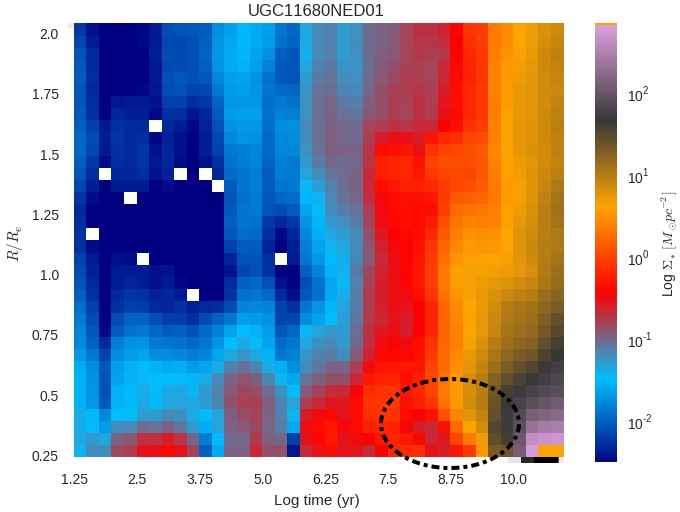
\includegraphics[scale=0.5]{figure_1.png}
  \caption[Densidad de masa estelar superficial, que define el mapa de Historia de Formación Estelar de UGC11680]{Densidad de masa estelar superficial, que define el mapa de Historia de Formación Estelar  de UGC11680. Se colocó un círculo punteado alrededor de la zona que tiene un ``corte'' en el gradiente de color, lo que implica un apagado que corre diagonalmente desde el centro galáctico hasta recorrer las zonas externas de la misma. Este corte no se observa en los promedios que se analizarán en la siguiente sección}
  \label{sfh_ugc11680}
\end{figure}


\noindent El resultado final, la historia de formación estelar espacialmente resuelta, dado por la densidad de masa estelar superficial o simplemente el mapa $SFH(t,R)$ para UGC11680, será el principal objeto de nuestro análisis. En la figura \ref{sfh_ugc11680}
el eje de las $X$ es la edad de las SSP a escala logarítmica, comienza con $\sim$ 14 Gyrs (la edad mas temprana de las SSPs utilizadas)
en el principio de la época cosmológica hasta el presente o tiempo actual que aquí definimos como tiempo cero.



\bigskip

\noindent Aunque no los utilizaremos, es interesante lo que muestran  las Figuras \ref{mass_SFH} y \ref{lum_SFH}. Estas muestran los mapas de la distribución espacial en luz (banda V) y densidad superficial de masa de la galaxia UG11680  para cada edad comprendida dentro de la plantilla SSSp utilizada. Si dividiéramos por el intervalo temporal tendríamos la tasa de formación estelar a cada tiempo. Se aprecia que a edades tempranas había mas formación estelar en el centro y más en las partes externas en edades recientes.



\begin{figure}
  \centering
    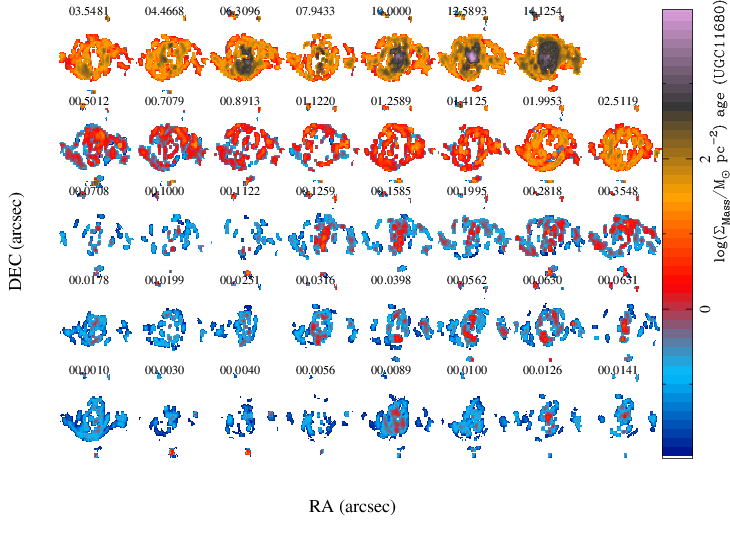
\includegraphics[scale=0.5]{Converted_file_73ee484d.png}
  \caption[Mapas de Densidad de masa superficial]{Mapas de densidad de masa estelar temporal cumulativa para UGC11680 antes de la compresión de los ejes $XY$ . La lectura de ellos comienza en la esquina superior derecha y termina en la esquina inferior izquierda}
  \label{mass_SFH}
\end{figure}

\noindent
\begin{figure}
  \centering
    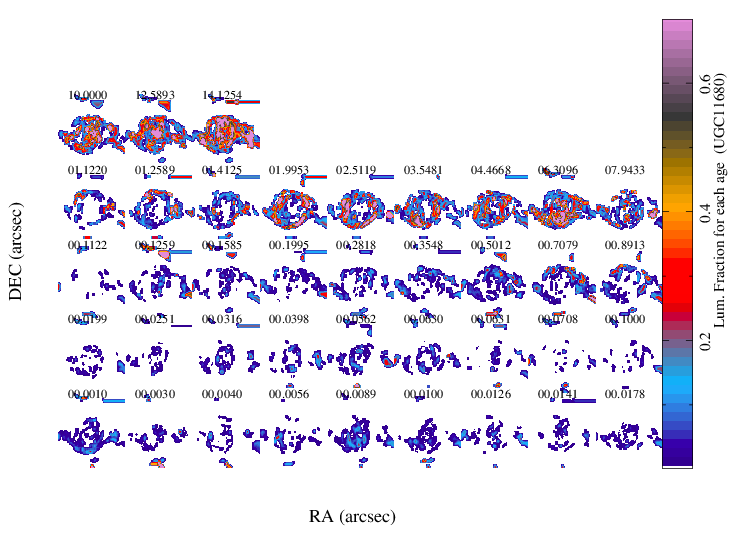
\includegraphics[scale=0.4]{18UGC11680_proc_elinesUGC11680_pruebas.png}
  \caption[Mapas de densidad superficial de luminosidad para UGC11680]{Disposición de mapas de luminosidad superficial para UGC11680 para cada SSP. Estos mapas temporales inician desde la esquina superior derecha y terminan en la esquina inferior izquierda.}
  \label{lum_SFH}
\end{figure}


\bigskip

\noindent Es importante aclarar que no existe acuerdo en la semántica de la palabra ``Historia'' en estudios de síntesis espectral. El mismo término puede ser utilizado de muchas formas en la literatura, siempre refiriéndose a alguna  medida de como la formación estelar evoluciona en el tiempo, pero cuantitativamente variando desde estimados en la edad promedio a mediciones de formación ``reciente'' (donde reciente puede ser cualquier cosa entre $\sim$ 10 Myrs a unos Gyrs, dependiendo de los trazadores). Además de las diferentes escalas de tiempo, diferentes índices pueden ser usados para medir la historia de formación estelar, tal como la luminosidad \citep{cid2013_1} o masa asociada a las estrellas dado un intervalo de edad, en forma cumulativa o diferencial, etc. Sin embargo, en este trabajo, siempre nos referiremos a la historia de formación estelar usando la densidad de masa estelar.

\bigskip


\noindent La riqueza de información de este mapa es de suma importancia y muestra claras diferencias entre galaxias o promedios de ellas; además, el mapa $SFH$ de la Figura \ref{sfh_ugc11680} nos da una representación bidimensional
de la producción de masa estelar en densidad de masa a tiempo dado. Las zonas menos densas representan desde una muy baja hasta nula formación estelar, mientras que las zonas más densas, sobre todo cerca del centro, nos da un un ensamblaje alto.

\bigskip

\noindent Observamos entonces que el mapa ya nos da indicios de ensamblaje ``dentro fuera'' para UGC11680. Marcamos con un círculo punteado la zona cerca de la parte central en donde se cambia de densidad, en forma de ``corte'' diagonal a edades tempranas $\sim$ 4 Gyrs (o altos \textsl{redshifts}) . Observamos también que la galaxia ensambló prácticamente toda su masa en aproximadamente $\sim$ 9 Gyrs.
Nótese también que la galaxia tiene moderados brotes de formación estelar en su centro y cerca de sus zonas medias,
y las partes externas prácticamente ya no forma estrellas a épocas actuales. Sin embargo, esto es un resultado cualitativo y corresponde al siguiente capitulo analizar la historia de formación estelar cuantitativamente.

\bigskip



\noindent En este capítulo se mostró que el polvo no enrojece lo suficiente a esta galaxia y que su tasa de formación estelar
esta por debajo de la secuencia principal de galaxias que forman estrellas.
Se analizó el proceso para obtener el mapa $SFH(t,R)$, es decir, la historia de formación estelar espacialmente resuelta de UGC11680.
En lo restante, analizaremos este mapa, comparándolo con diferentes mapas promediados, para que cualitativamente,
decidamos en cual de estos encaja mejor y así dar algunas hipótesis del apagado estelar.









 % The \citep command functions as follows:
 %   \citept{key} ==>>                Jones et al. (1990)
 %   \citept*{key} ==>>               Jones, Baker, and Smith (1990)
 %   \citepp{key} ==>>                (Jones et al., 1990)
 %   \citepp*{key} ==>>               (Jones, Baker, and Smith, 1990)
 %   \citepp[chap. 2]{key} ==>>       (Jones et al., 1990, chap. 2)
 %   \citepp[e.g.][]{key} ==>>        (e.g. Jones et al., 1990)
 %   \citepp[e.g.][p. 32]{key} ==>>   (e.g. Jones et al., p. 32)
 %   \citepauthor{key} ==>>           Jones et al.
 %   \citepauthor*{key} ==>>          Jones, Baker, and Smith
 %   \citepyear{key} ==>>             1990





%%%%%%%%%%%%%%%%%%%%%%%%%%%%%%%%%%%%%%%%%%%%%%%%%%%%%%%%%%%%%%%%%%%%%%%%%
%                          Descripción de la planta                     %
%%%%%%%%%%%%%%%%%%%%%%%%%%%%%%%%%%%%%%%%%%%%%%%%%%%%%%%%%%%%%%%%%%%%%%%%%






%%%%%%%%%%%%%%%%%%%%%%%%%%%%%%%%%%%%%%%%%%%%%%%%%%%%%%%%%%%%%%%%%%%%%%%%%
%                          Modelado                                     %
%%%%%%%%%%%%%%%%%%%%%%%%%%%%%%%%%%%%%%%%%%%%%%%%%%%%%%%%%%%%%%%%%%%%%%%%%

%%%%%%%%Tabla Nombres de parámetros



%%%%%%%%%%%%%%%%%%%%%%%%%%%%%%%%%%%%%%%%%%%%%%%%%%%%%%%%%%%%%%%%%%%%%%%%%
%                          Subsección
%%%%%%%%%%%%%%%%%%%%%%%%%%%%%%%%%%%%%%%%%%%%%%%%%%%%%%%%%%%%%%%%%%%%%%%%%
      % ~20 páginas - Explicar el problema en específico que se va a resolver, la metodología y experimentos/métodos utilizados
\chapter{Análisis de Resultados}

\lettrine[lines=1]{U}n método para investigar que sucedió con la galaxia UGC11680, es interpretar
la información que nos provee su  historia de ensamblaje de masa estelar, analizando los datos que se obtienen del mapa $SFH$, ya que esto nos dará claves para saber si su apagado fue un proceso de dentro hacia afuera ó viceversa. Para esto, nos interesará saber si la historia de formación estelar se parece a algún tipo de historia  promediada de otras galaxias o tipos de galaxias.

\bigskip

\noindent Así mismo,  podemos comparar con promedios de diferentes tipos de galaxias, dada la característica principal de la galaxia UGC11680: con el promedio de los AGNs tipo dos, y con promedios en categorías color-masa. Estos promedios se contrastan con la galaxia que estamos estudiando y ver en donde ajusta o difieren.
Esto tiene implicaciones inmediatas: en la literatura astronómica no existe esta clase de comparaciones, por lo que en si misma, ofrece
una metodología nueva gracias a la espectroscopía de campo integral y sus mapas  $SFH(t,R)$

\section{Los Datos y sus Promedios}

\noindent Se utilizaron 574 mapas $SFHs$ de la muestra de \textbf{CALIFA} y se dividieron en los siguientes grupos:

\begin{itemize}

  \item En 24 AGNs de tipo 2 de la muestra, sin importar su morfología.

  \item Los 574 SFH divididos por categorías de color-masa, para simular el diagrama color-masa de galaxias, pero con mapas $SFHs$. Esta clasificación es de suma importancia ya que estudios anteriores muestran que la masa es fundamental para determinar el tipo de crecimiento en galaxias.

\end{itemize}

\noindent Detallando más las categorías, se dividieron las 574 $SFH$ de cada galaxia en cuatro bines de masa. Una vez dividido, a su vez esas categorías se dividieron por color. El número de galaxias en cada categoría se muestran en la Tabla \ref{tab_CMD}. Para cada división, se utilizó su mapa $SFH(t,R)$.

\bigskip



\noindent Es importante señalar que excluimos los bines de menor masa y color por tener un sólo objeto y por lo tanto no tener importancia estadística. Así mismo, la zona de las galaxias más rojas y masivas ($\sim 10^{11.5} M_{\odot}$) contiene solo 6 mapas $SFH$, pero lo mantendremos por la importancia comparativa  con la galaxia de estudio. Por último, a pesar de que separamos los AGNs para su análisis, estos mismos fueron incluidos en su categoría color-masa correspondiente. UGC11680 se excluyó del promedio de los AGNS, pero se incluyó en su categoría correspondiente en color-masa ($3 \le g-r \le 4$ ; $11 \le M_{\odot} \le 12$)
.

\begin{figure}
  \centering
    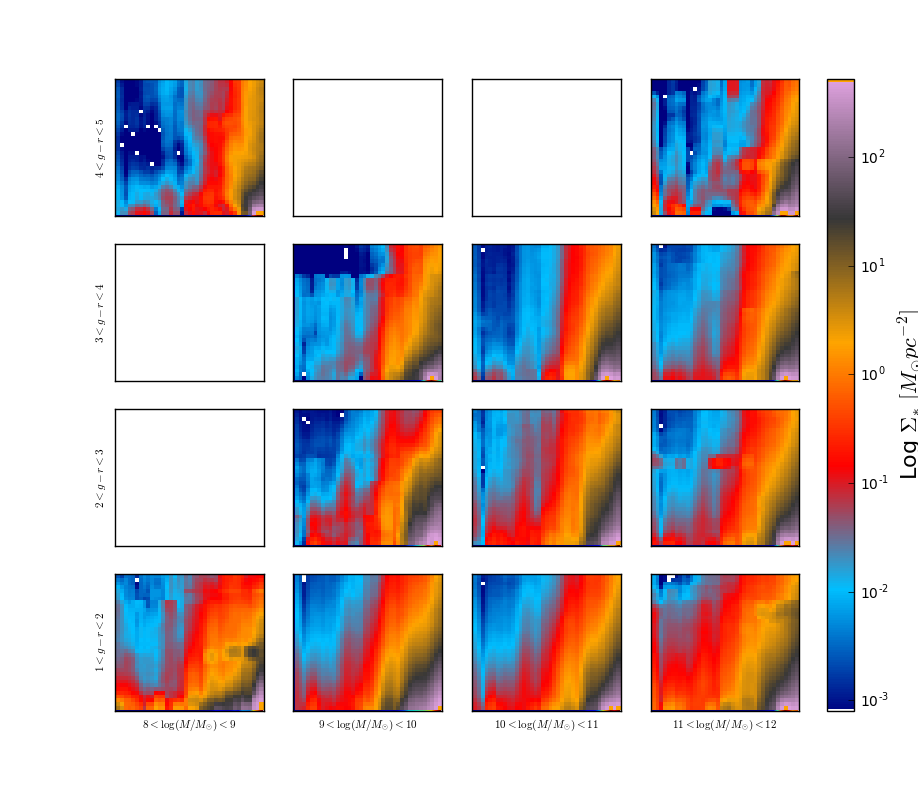
\includegraphics[scale=0.6]{cmd_sfh.png}
  \caption[Diagrama Color-Masa para la muestra de CALIFA]{Diagrama Color-Masa  para las $SFH(t,R)$ pertenecientes a su intervalo correspondiente.
           Cada $SFH(t,R)$ de la muestra de  \textbf{CALIFA} individual fue promediado con todos los de su categoría,
           por lo que cada una de ellas muestra un promedio para el intervalo de color-masa correspondiente. En la esquina superior izquierda, esta el mapa de UGC11680, por comparación.La cantidad de galaxias para cada categoría están dados en la tabla \ref{tab_CMD}. Las escalas temporales y radiales son las mismas que se dieron para mapas de galaxias individuales.Nótese el ensamblaje más grande para galaxias más masivas, además del lento ensamblaje de las galaxias más ligeras, además del apagado de UG11680, mas notorio debido al escalamiento.}
  \label{CMD}
\end{figure}



\begin{table}[!ht]
\centering
\begin{tabular}{||c | c | c | c | c||}
\hline
\hline
Color  / $\log$ Masa & $8< M_{\odot} < 9$ & $9< M_{\odot}< 10$ & $10< M_{\odot}< 11$ & $11< M_{\odot}< 12$ \\
\hline
\hline
$0< (g-r)<1$ & 1 & 1  & -- & -- \\

$1< (g-r)<2$ & 8 & 15 & 18 & 28 \\

$2.< (g-r)<3$ & -- & 63 & 114 & 67 \\

$3< (g-r)<4$ & -- & 87 & 70 & 96\\

$4< (g-r)<5$ & -- & -- &-- & 6\\
\hline
\hline
\end{tabular}
\caption{Disposición de las galaxias de la muestra de acuerdo a su color y masa. Las partes vacías pertenecen a categorías que no contenían objetos en la muestra.}
\label{tab_CMD}
\end{table}

\section{Promedios de los $SFH(t,R)$}

 El promedio por categoría $SFH_{cat}$ está dado por la definición clásica


\begin{equation}
\left<SFH_{cat}(t,R)\right> = \frac{1}{m}\sum_{i=1}^{m} SFH_{i} (t,R)
\end{equation}

\begin{figure}[htbp]
\centering
\subfigure[UGC11680]{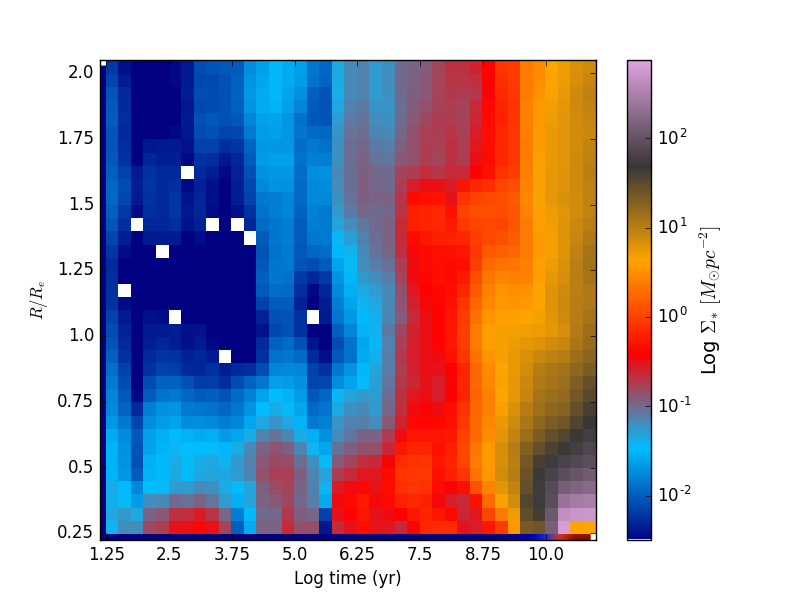
\includegraphics[width=80mm]{sfh_map_ugc11680.png}}
\subfigure[Todos los AGNs Promediados]{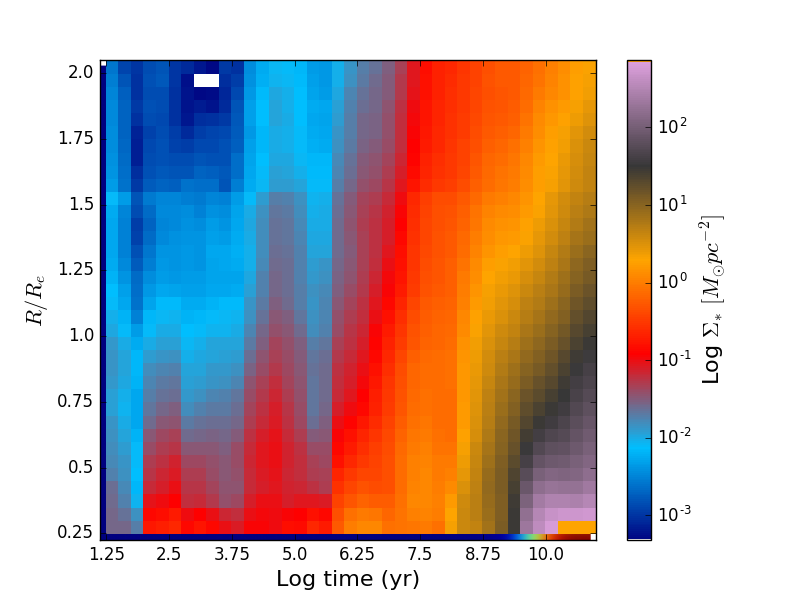
\includegraphics[width=80mm]{all_agns_mgh.png}}
\caption[Historias de Formación estelar, para UGC11680 y AGNs]{Historias de Formación estelar, para UGC11680  y AGNs tipo 2. Comparando cada mapa, ya es clara la diferencia entre UGC11680 y este promedio, ya que UGC11680 muestra un abrupto cambio en su densidad de masa estelar, en forma de corte diagonal, que parte de su centro y que comienza en $\sim$ 10 Gyrs. Nótese también en ensamblaje de dentro hacia afuera de los 3 mapas.}
\label{all_agns_sfh}
\end{figure}


\noindent Entonces, el $SFH_{cat}(t,R)$ es la suma  de $i-$ objetos en cada categoría.
Por ejemplo, para el caso del grupo de AGNs, $cat$= AGNs y m=24 el número de $SFHs$
en este grupo. Análogamente, consideramos cada categoría en la selección de galaxias por color-masa.
El paso siguiente seria entonces definir parámetros que nos den información
para comparar  el $SFH_{cat}$ para los diferentes promedios con la galaxia UGC11680. Estos promedios, junto con la $SFH$ de UGC11680 se muestran en las Figuras \ref{CMD} y \ref{all_agns_sfh}.
\bigskip

\noindent En la Figura \ref{CMD} podemos apreciar  como la masa determina en gran medida la rapidez de ensamblaje de la densidad estelar (e.g., \citep{perez2013}; \citep{perezg2008}) ;({\color{red} Ibarra-Medel, et al. Submitted }) . El mapa  $SFH$ de la galaxia UGC11680 se colocó en la esquina superior izquierda para su comparación y referencia. Notamos que para galaxias  más masivas, el ensamblaje de masa  es más rápido. También observamos que las galaxias menos masivas  es notorio que en promedio todavía siguen formando estrellas a edades actuales. Ahora, en la Figura \ref{all_agns_sfh} vemos que los AGNs carecen del corte diagonal que existe en el mapa $SFH$ de UGC11680, así como las diferentes densidades que muestra la espiral roja, sobre todo en las partes medias y externas. Nótese igualmente que aunque los AGNs no muestran ese corte tan notorio como UGC11680, si muestran una evolución temporal de densidad de masa estelar más abrupto que UGC11680.



\section{Parámetros Analizados}

En esta sección obtendremos parámetros básicos para el análisis de $SFHs$ ya sean individuales o de promedios.
Estos parámetros ya han sido analizados anteriormente en la literatura sobre galaxias
espacialmente resueltas, tal como en \citet{cid2013_1} \cite{perez2013} y \citet{gonzalezdelgado2016} {\color{red} Ibarra-Medel, et al. (Submitted) }. En nuestro caso, estos parámetros son importantes ya que nos dirán si la galaxia de nuestro estudio creció de dentro hacia afuera y si detuvo su formación estelar. De esta forma, al compararla con los promedios sabremos si su comportamiento es atípico para galaxias con sus características o es algo común en el grupo seleccionado.


\subsection{Perfil Radial de Densidad de Masa Estelar ($PR \Sigma_{*}$) }

A partir del mapa $SFH$ también podemos calcular la densidad de masa acumulada radialmente a cualquier tiempo/edad dada su distancia radial normalizada al radio efectivo ($R/R_e$). Para esto, definimos su perfil radial de densidad de masa estelar acumulada $PR \Sigma_{*}$ como

\begin{equation}
PR \Sigma_{*}= \sum_{t=1}^{n_t} SFH(t,R)
\end{equation}



\noindent Donde $n_{t}$ es la dimension temporal de la imagen. Este perfil nos da información de como se acumuló masa a diferentes radios, desde las partes centrales hasta las afueras. Así mismo, se podría integrar la formula a todo tiempo y sacar un $PR \Sigma_{*}$ promedio actual para la galaxia en cuestión. Los valores esperados de esta acumulación de masa serían gradientes con pendiente negativa conforme nos alejaremos de las zonas centrales y en el caso de una disminución de acumulación de masa estelar el cambio sería a un gradiente de pendiente positiva ó plana. El resultado se muestra en la Figura \ref{perfil_radial}. Se dividió en 4 épocas cosmológicas, para una comparación más sencilla.

\bigskip

\noindent Observamos que los AGNs tipo 2 muestran la caída típica (indicador de una formación dentro-fuera) desde las zonas centrales a las afueras de estas galaxias. Esto se repite para cada época cosmológica seleccionada. Esta acumulación de masa es mayor en las partes centrales que en las partes medias, así como las afueras de estas. La acumulación de masa es mayor de dentro hacia afuera. Ahora, para la espiral roja notamos que a épocas $\sim$ 14Gyrs tiene una acumulación de masa mayor en las partes centrales que va cayendo conforme se aproxima a sus zonas externas. Sin embargo, esta acumulación cambia su gradiente en las partes centrales tanto en $\sim 12$ Gyrs como en $\sim$ 8 Gyrs. Esto nos indica que UGC11680 dejó de acumular masa en esas zonas para después tener la caída típica hacia las afueras que vuelve a cambiar en las zonas medias, para caer finalmente en las partes externas. Estos cambios se notan en $z \sim 0$ en la parte media. Esto cambios de pendiente implican que la galaxia roja efectivamente tiene a diferentes épocas momentos en que  ensambla masa, pero vuelve a tener caídas de acumulación con respecto a los promedios. Algo parece regular la acumulación de masa, y que es un proceso que comienza en las partes centrales.






\begin{figure}[htbp]
\centering
\subfigure[UGC11680]{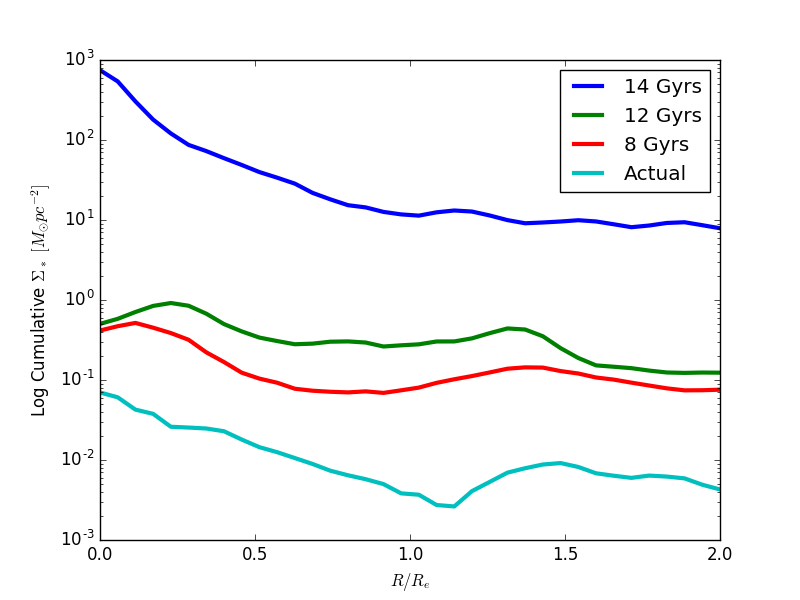
\includegraphics[width=60mm]{ugc11680_pr.png}}
\subfigure[AGNs]{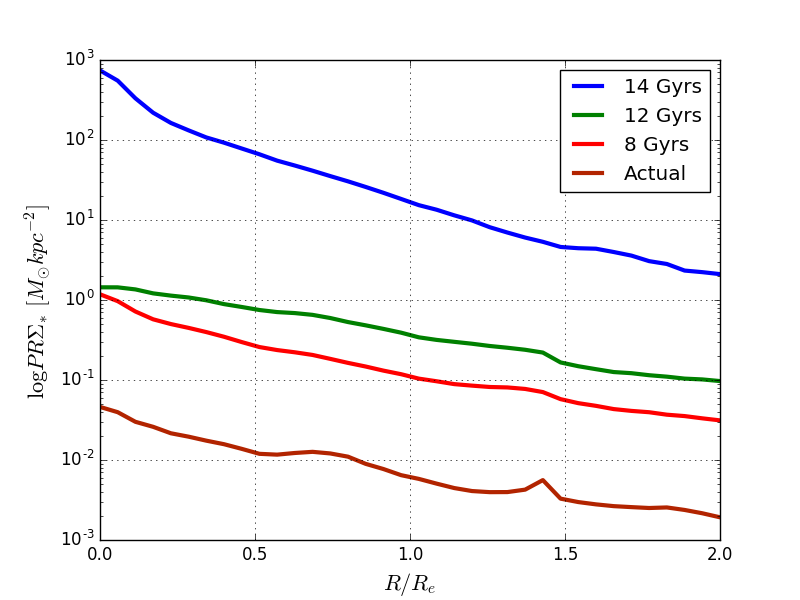
\includegraphics[width=60mm]{radial_all_agns.png}}
\caption[Perfil radial de masa estelar cumulativa de UGC11680 y AGNs]{Perfil Radial de densidad de masa superficial cumulativa de UGC11680 y los AGNs tipo 2. Cada color muestra diferentes épocas, escogidas para una mejor disposición visual. El aplanamiento en el gradiente de densidad radial para la espiral roja en épocas intermedias, mientras que los AGNs mantienen un gradiente una densidad de masa estelar casi constante en su historia de formación estelar}
\label{perfil_radial}
\end{figure}



\subsection{Historia de Crecimiento de Masa ($HCM(t)$)}

\begin{figure}[htbp]
\centering
\subfigure[UGC11680]{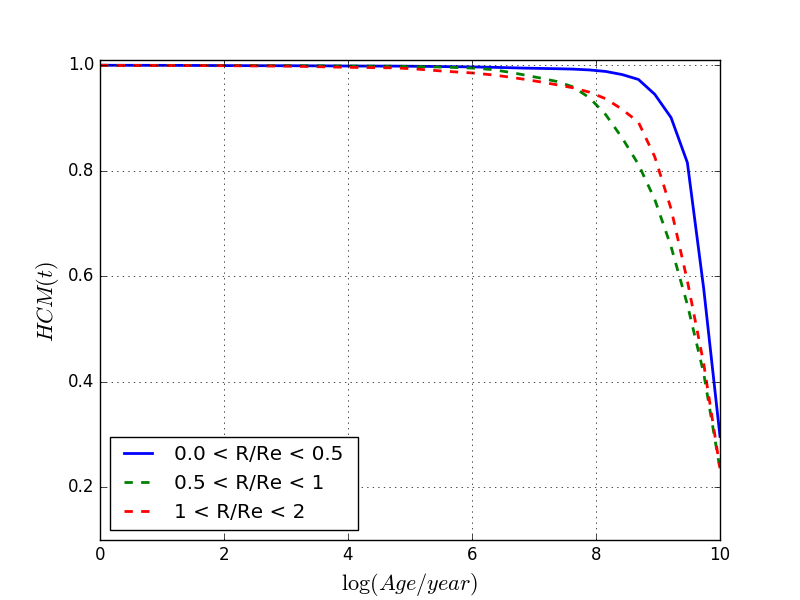
\includegraphics[width=60mm]{ugc11680_mgh.png}}
\subfigure[AGNs]{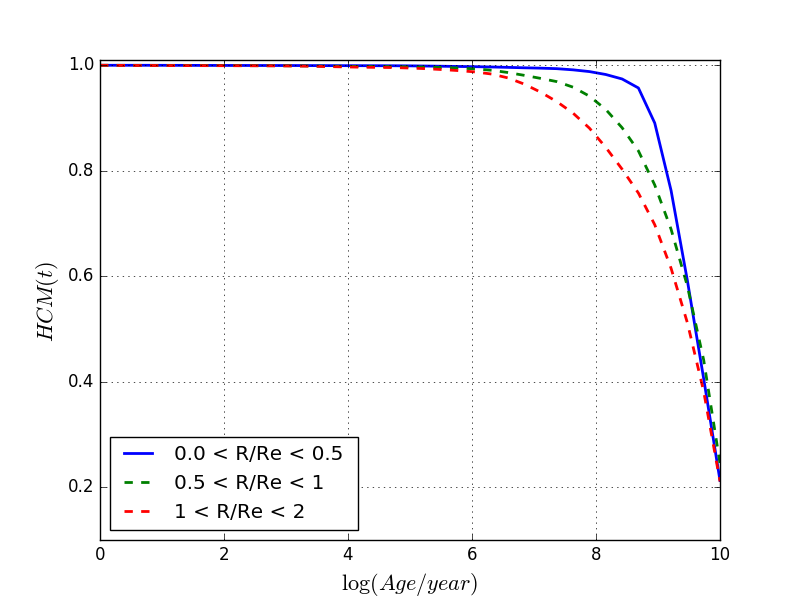
\includegraphics[width=60mm]{all_agns_mgh_log.png}}
\caption[MGHs para UGC11680 y AGNs]{Gráfica de ensamblaje de masa cumulativa de UGC11680 y los AGNs tipo 2. La línea azul corresponde a la parte central medida por su radio efectivo, la verde a la parte media y la roja a las afueras, normalizadas a la masa actual. Aunque no es concluyente para el apagado, si lo es para demostrar que UGC11680 y los AGNs ensamblaron su masa de dentro hacia afuera.}
\label{ensamblaje_log}
\end{figure}

\bigskip

\noindent Siguiendo la misma línea de razonamiento,  tomamos el mapa $SFH(t,R)$ para ahora ver el crecimiento acumulativo de la masa estelar $M_{*}$. Esto nos indicará si el crecimiento es de dentro hacia afuera a escala temporal (a diferencia del parámetro de la sección anterior, que fue dependiente del radio) o viceversa, así como el apagado, (si es que existiera) en su formación estelar. Definimos entonces la historia de crecimiento en masa como la masa relativa al total $M(t)/M_{T}$. Este parámetro normalizado contiene 39 intervalos de tiempo, por lo que obtenemos la $HCM(t)$ o historia cumulativa de masa como

\begin{equation}
HCM(t)= \frac{1}{M(T)} \sum_{R=1}^{n_R} SFH(t,R) + M(t-1)
\end{equation}

\noindent Donde

\begin{equation}
M_{T}= \sum_{R=1}^{n_R} \sum_{t=1}^{n_t} SFH(t,R)
\end{equation}

\bigskip

\noindent  $HCM(t)$  es la masa estelar relativa acumulada al tiempo $t$ y donde $n_t$ y $n_R$ son las dimensiones temporal y espacial, respectivamente. Por lo tanto, esta definición cuantifica la cantidad de masa estelar que se acumula durante la evolución de la galaxia. De esta forma podemos obtener diferentes historias de acumulación masa a lo largo de la distribución radial, simplemente integrando sobre diferentes regiones determinadas por el radio efectivo. Como nuestros mapas tienen 36 intervalos de radio normalizado, integraremos en 3 partes de 12 intervalos cada uno, a menos de que se especifique lo contrario. A diferencia del perfil radial, esta gráfica nos indica la acumulación en el tiempo, comparada con su masa final a diferentes radios efectivos. Un perfil con pendiente mas inclinada nos dará las zonas en donde ensambló primero su masa. El resultado se muestra en la Figura \ref{ensamblaje_log}.

\bigskip

\noindent Observamos que en los dos casos ya podemos decir que para los AGNs y UGC11680 el crecimiento en todos los casos es de dentro hacia afuera dado que la línea azul que representa la parte central, tiene la pendiente más pronunciada, (Al menos desde los últimos 3-4 Gyrs) seguido por sus partes medias y terminando en sus afueras, algo observado por \citet{perez2013} y por {\color{red} Ibarra-Medel, et al. (Submitted) }, por ejemplo. Obsérvese también que en los dos casos, el ensamblaje de su masa final termina en $\sim$ 1 Myr. Sin embargo, la bondad de la escala logarítmica-temporal para determinar el crecimiento dentro-fuera, carece de detalle para saber si existió un apagado en su acumulación masa. Para eso simplemente cambiamos el tiempo a escala lineal, este cambio se muestra en la Figura \ref{ensamblaje_lineal}.


\begin{figure}[htbp]
\centering
\subfigure[UGC11680]{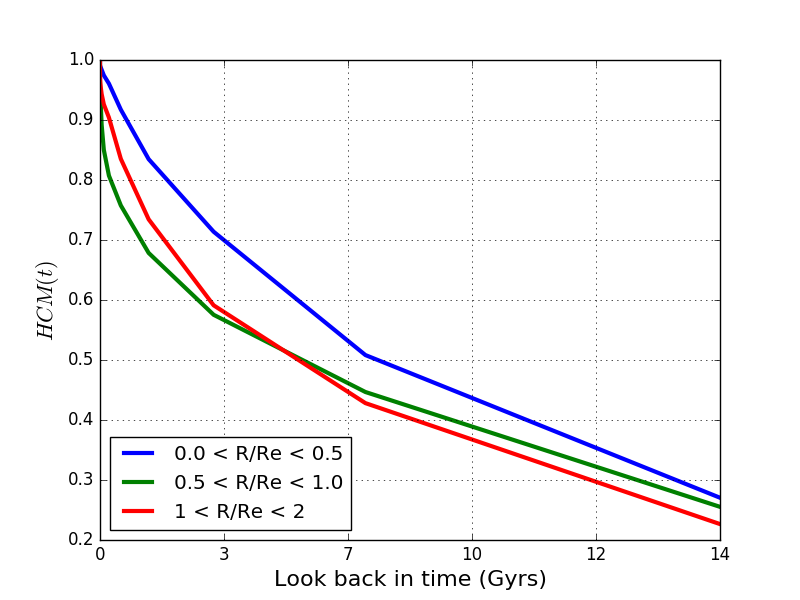
\includegraphics[width=60mm]{ugc11680_mgh_lineal.png}}
\subfigure[AGNs]{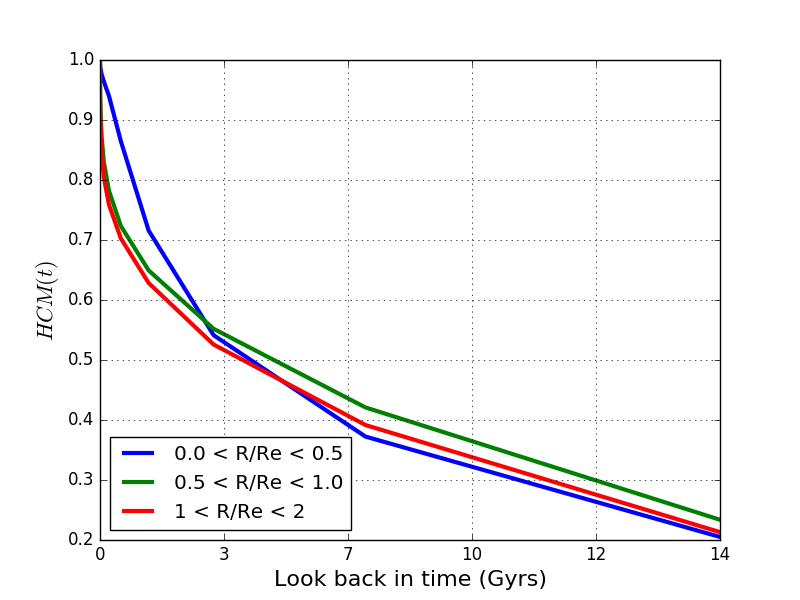
\includegraphics[width=60mm]{all_agns_mgh_lineal.png}}
\caption[Historia de Crecimiento de Masa con tiempo lineal, UGC11680 y AGNs tipo 2]{Gráfica de Ensamblaje de masa cumulativa de UGC11680 y AGNs tipo 2, con los mismos colores que la figura \ref{ensamblaje_log} pero hora a una escala temporal lineal. Nótese que ya es evidente el apagado en formación estelar comparado con los otros promedios. Esta gráfica y la figura \ref{ensamblaje_log} ya son muestran del apagado de dentro hacia afuera de UGC11680.}
\label{ensamblaje_lineal}
\end{figure}



\noindent Estas figuras ya muestran diferentes resultados según se observen los promedios ó la galaxia UGC11680. Para esta última vemos que en todo momento, la galaxia ensambla su masa desde el centro hacia afuera, es decir, un crecimiento ``dentro-fuera''. Sin embargo algo sucede en épocas $\sim$ 6 Gyrs: el ensamblaje se vuelve mas lento con respecto a las afueras, hasta que finalmente se ensambla primero la masa estelar en las afueras de la galaxia para finalmente terminar con las partes medias. Parece ser entonces que la zona media detiene (pero no completamente) su ensamblaje de masa estelar.En el caso de UGC11680, esta ensambla el 50\% de su masa estelar a $\sim$ 4 Gyrs y finalmente el promedio de los AGNs a  $\sim$ 3 Gyrs.

\bigskip

\noindent Podemos decir entonces que la galaxia espiral roja, en todo momento, ensambla su masa estelar desde dentro hacia afuera, pero las partes centrales pierden intensidad en la acumulación de masa frente a las partes externas hasta que  estas ensamblan primero su masa estelar antes que las partes medias. Esto junto con el perfil radial de densidad de masa analizado en la sección anterior, así como el mapa $SFH$ nos dicen que el ensamblaje de masa estelar de UGC11680 muestra que las zonas tanto centrales como medias detuvieron parcialmente su ensamblaje, aún frente los AGNs promediados. En todos los casos, el crecimiento es de dentro hacia fuera en ciertas épocas cosmológicas.



\subsection{Distribución Radial de la Densidad Superficial de la Tasa de Formación Estelar}

\begin{figure}[htbp]
\centering
\subfigure[UGC11680]{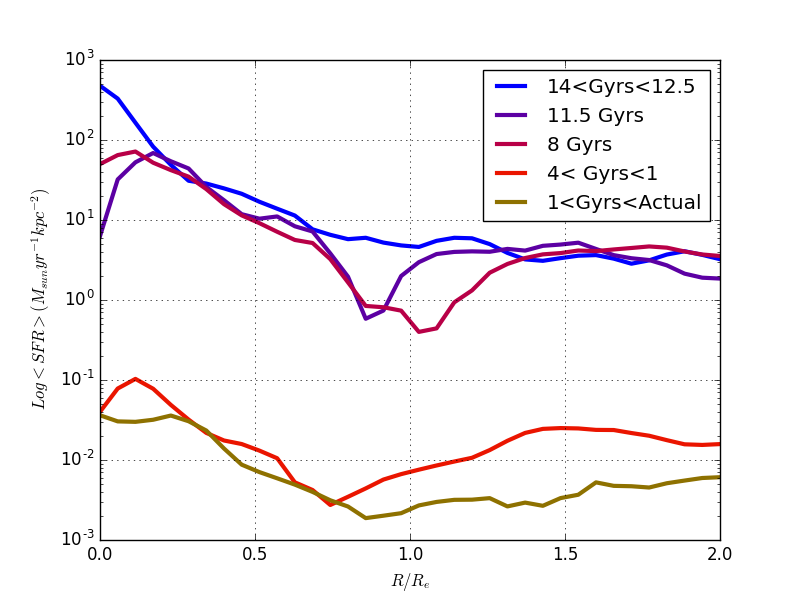
\includegraphics[width=70mm]{ugc11680_sfr.png}}
\subfigure[AGNs]{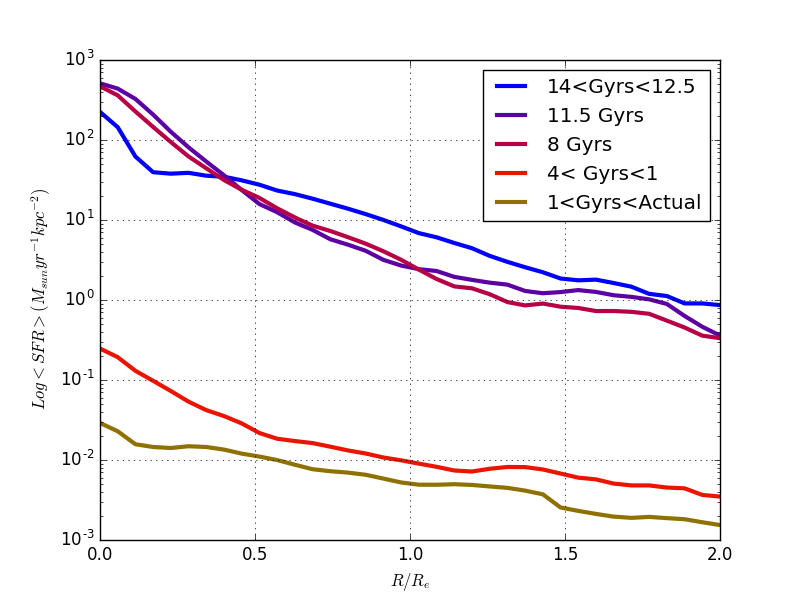
\includegraphics[width=70mm]{all_agn_sfr.png}}
\caption[Tasas De formación Estelar Radiales]{Distribución Radial de la densidad de formación estelar a diferentes edades para la galaxia de estudio, UGC11680  y los AGNs.}
\label{sfr}
\end{figure}


\noindent Como se mencionó anteriormente, podemos obtener la tasa de formación estelar a cada edad cosmológica ó a cada tiempo con ayuda de el mapa $SFH$. Esta se calcula como el cambio en masa estelar con respecto al tiempo, es decir

\begin{equation}
SFR(R)= \frac{\Delta SFH(t,R)}{\Delta t}
\end{equation}


\noindent El resultado de esta ecuación para distintos tiempos se muestra en la Figura \ref{sfr}. La interpretación de la gráfica es muy parecida a la de perfil radial, donde igualmente se consideran diferentes épocas cosmológicas para mayor interpretación visual, solo que para este caso hablamos de una tasa de formación y no una acumulación de masa estelar. Así, la $SFR$ temporal nos corrobora lo obtenido con los otros parámetros de acumulación de masa, tanto radial como temporal-porcentual: UGC11680 detuvo su formación estelar comenzando en las zonas centrales (El cambio a pendiente negativa). Sin embargo, la $SFR$ temporal nos da un resultado mas sutil: este apagado no es algo constante y sostenido, sino que aparece y desaparece dependiendo de la época cosmológica considerada. Esto implica que más que un apagado constante, la parte central aparecen eventos secuenciales de apagado y encendido, en lugar de detener completamente la formación estelar en el caso de UGC11680, lo que no se aprecia con el mapa $SFH$ de esta galaxia. Nótese además que a épocas cosmológicas actuales, prácticamente en todos los grupos de galaxias, la producción de estrellas es baja, y que en todos los casos la caída de la SFR es pronunciada en las partes externas, aunque UGC11680 tiene ligeros brotes de formación en las partes medias que ya habían notado en los otros parámetros así como en la inspección visual.

\bigskip

\noindent Podemos decir que estos tres análisis combinados, ya nos dicen que el comportamiento de UGC11680 es atípico con respecto a los promedios utilizados. los perfiles radiales nos dicen que efectivamente, se detuvo la formación estelar en las partes centrales, aunque no de manera sostenida. El perfil temporal nos dice que este proceso es dentro hacia afuera. Es decir. la masa y el AGN son algo fundamental en este proceso. Ahora podemos preguntarnos, ¿Que tan atípico es con respecto a los promedios que se utilizaron? Esto nos permitirá saber si la $SFH$ encaja en con algún otro promedio de galaxias y por lo tanto determinar a que grupo de galaxias pertenece su historia de formación estelar.




\section{Comparación y ajuste usando la distribución $\chi^{2}_{\nu}$}

Una vez analizados los parámetros para la galaxia UGC11680 y los diferentes promedios, podemos
comparar el $SFH$ de  UGC11680  con los demás $SFH's$ promediados por categorías. Esto nos dirá estadísticamente a que grupo de los clasificados con anterioridad encaja mejor esta galaxia, en función de su mapa $SFH$. Esto es importante ya que comparamos historias de formación estelar, además de que esto nos dirá (en promedio) como ha sido la evolución de ensamblaje estelar de las demás de la muestra.

\bigskip


\noindent Entonces para poder hacer una comparación cuantitativa entre $SFHs$ utilizamos el parámetro $\chi^{2}_{\nu}$ que representa un valor $\chi^{2}$ reducido por el número de grados de libertad. Para nuestro caso, la dimensión de la imagen determinará estos grados de libertad con los que se va a dividir la $\chi^{2}$. Como la dimensión de nuestros mapas en el espacio radial es 36 (dado por el radio normalizado al radio efectivo) mientras que en el espacio temporal es 39 (dados por las SSPs), los grados de libertad serían  $36 \times 39$. De esta forma, definimos la $\chi^{2}_{\nu}$ para cada galaxia con respecto a la categoría a la que pertenecen como




\begin{figure}[htbp]
\centering
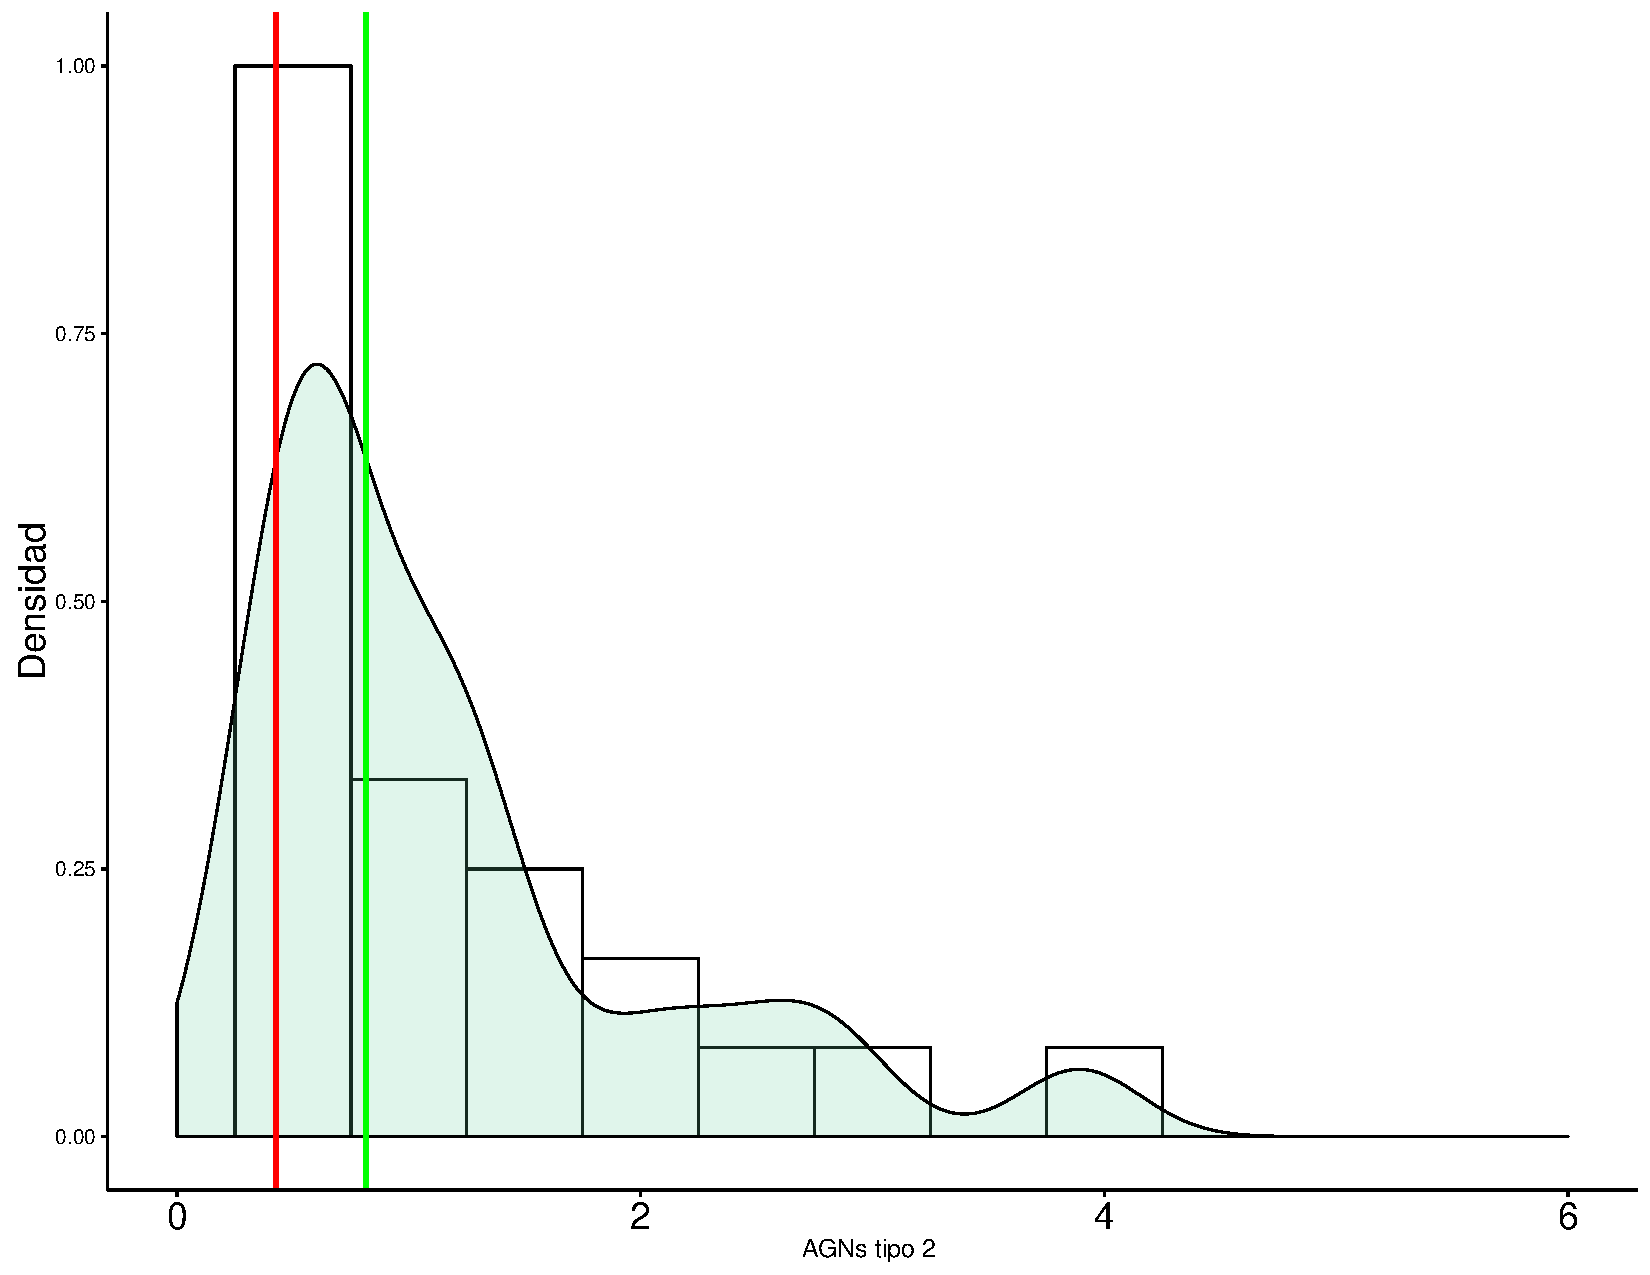
\includegraphics[width=90mm]{chi_agns.pdf}
\caption[Distribuciones $\chi^2_{\nu}$ para AGNs tipo 2] {Distribuciones $\chi^{2}_{\nu}$ los AGNs tipo 2 en la muestra. La línea roja corresponde a la $\chi^{2}_{\nu}$ de UGC11680 con respecto a la categoría señalada. La línea verde corresponde a la media de la distribución para esta categoría}
\label{ensamblaje_cara}
\end{figure}


\begin{figure}
  \centering
    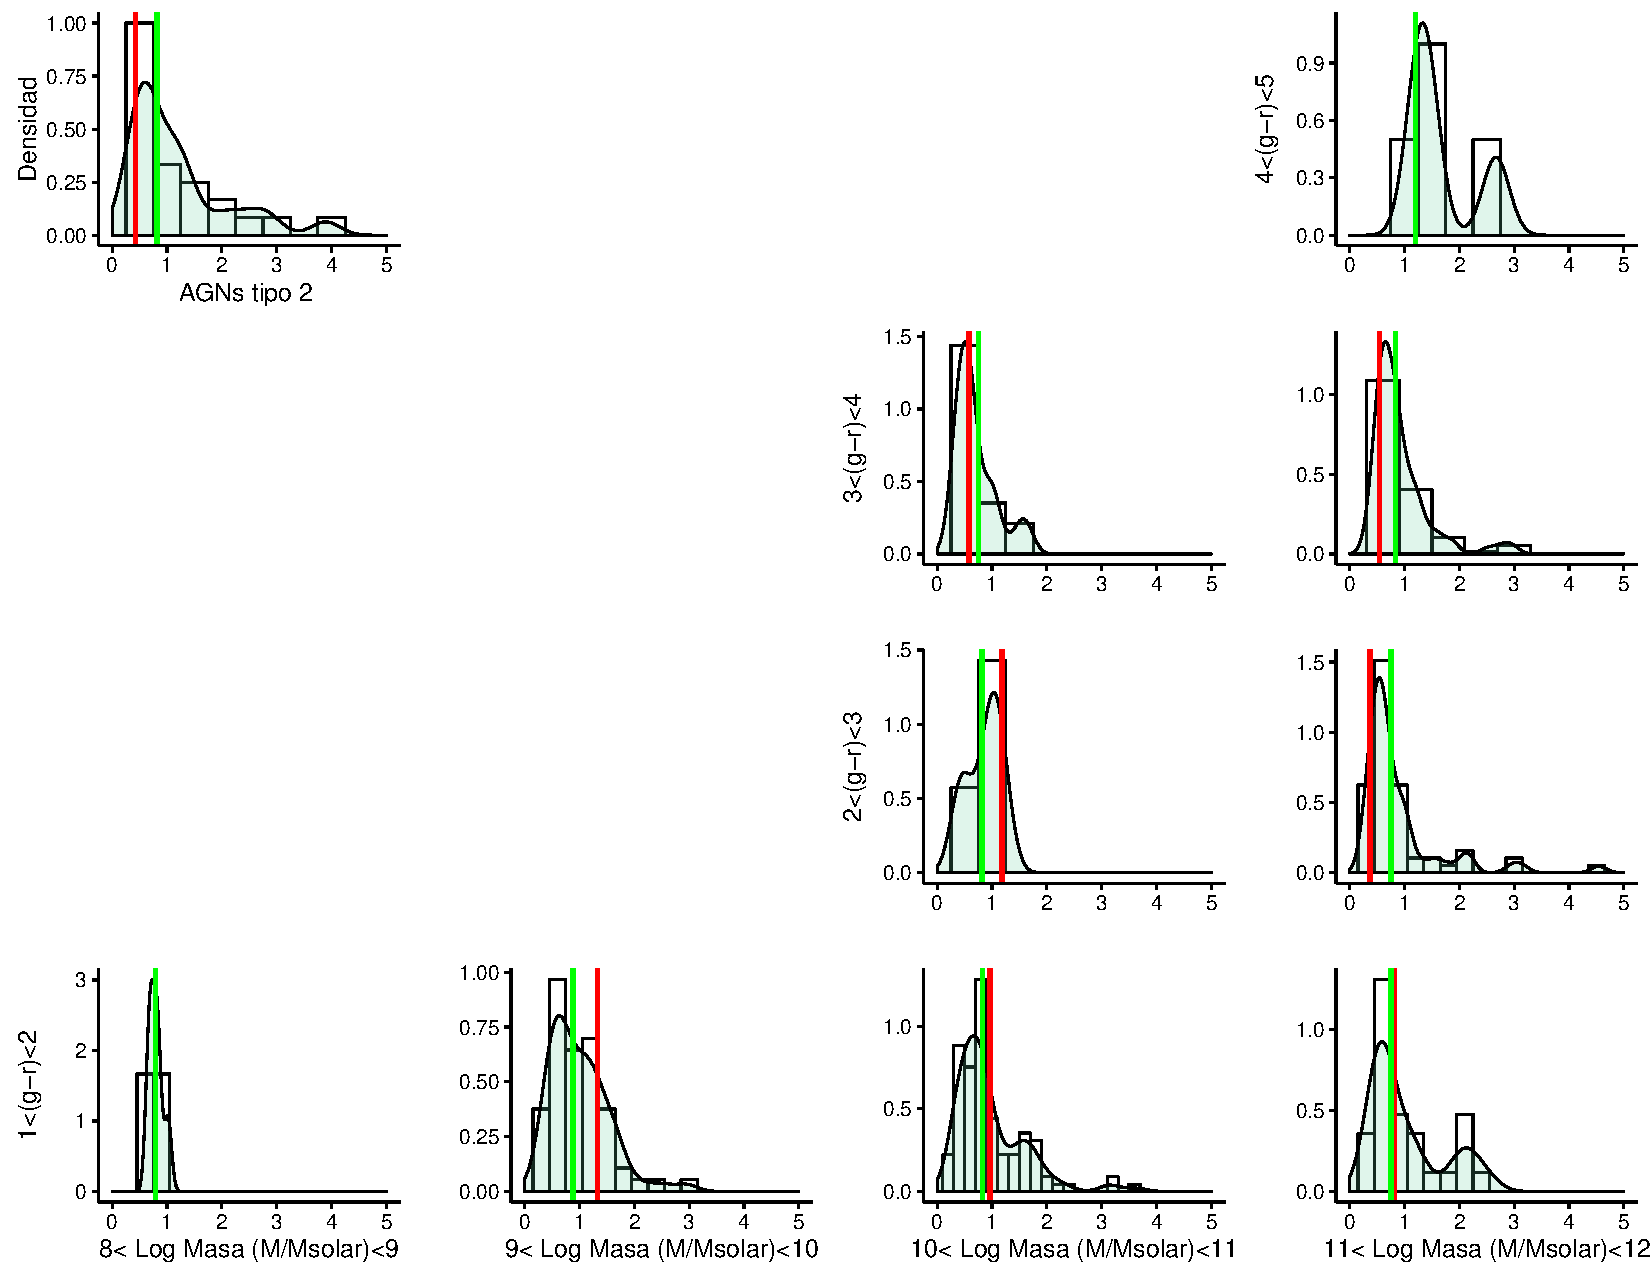
\includegraphics[scale=0.5]{exp_chi_perl.pdf}
  \caption[Diagrama de distribuciones $\chi^{2}_{\nu}$ en Color-Masa ]{Representación del Diagrama Color-Masa  con las distribuciones $\chi^2_{\nu}$ pertenecientes a su intervalo correspondiente.Cada distribución $\chi^2_{\nu}$ de la muestra de  \textbf{CALIFA}. La línea roja es la $\chi^2_{\nu}$ de UGC11680 para cada una de su categoría y la línea verde corresponde a la media de las distribuciones.En la esquina superior izquierda se colocaron las $\chi^2_{\nu}$ de los AGNs tipo 2 como referencia referencia }
  \label{chi_todos_mean}
\end{figure}




\begin{equation}
\chi^{2}_{\nu} = \frac{1}{2} \sum_{t=1}^{n_t} \sum_{R=1}^{n_R}  \frac{ \left[SFH_{data}(t,R)- \left <SFH_{cat}(t,R) \right > \right]^2}{\sigma(t,R)_{cat}^2}
\end{equation}

\bigskip

\noindent Donde $n_t$ , $n_R$ son las dimensiones temporales y radiales respectivamente, $SFH_{data}(t,R)$ es el flujo de la imagen a comparar ($\Sigma_{*}$, para los mapas $SFH$); $\left <SFH_{cat}(t,R)\right >$ es el mapa promedio definido anteriormente y finalmente  $\sigma(t,R)_{cat}^2$ es el mapa de dispersión de los datos por cada categoría definido como

\begin{equation}
\sigma(t,R)^2= \frac{1}{m-1} \sum_{i=1}^{m} \left[SFH_{i}(t,R)- \left <SFH_{cat}(t,R) \right > \right]^2.
\end{equation}


\bigskip

\noindent Una vez definido el parámetro $\chi^{2}_{\nu}$ lo usamos para definirlo en cada galaxia de la muestra  con respecto al promedio de su categoría. La $\chi^{2}_{\nu}$ de UGC11680 se colocó por separado para fines comparativos, así obtenemos 575 $\chi^{2}_{\nu}$ y 25 para la categoría de los AGNs. Estas $\chi^{2}_{\nu}$ se usan para su distribución con la categoría correspondiente y estas se muestran en la Figura \ref{ensamblaje_cara} que es el caso de la distribución de las $\chi^{2}_{\nu}$ para los AGNs tipo 2 y donde la $\chi^{2}_{\nu}$ de UGC11680 se muestra con una linea roja y la media con una línea verde, para comparaciones posteriores.

\bigskip

\noindent Estas distribuciones pueden ser también mostradas construyendo un diagrama que simule el diagrama color-masa para galaxias, como  se muestran en la Figura \ref{chi_todos_mean}, donde como en el caso anterior, se representa la $\chi^{2}_{\nu}$ de UGC11680 con una línea roja y la media con una línea verde. En la esquina superior izquierda colocamos la distribución de los AGNs para referencia. Nótese que se obtuvieron distribuciones  asimétricas, lo que concuerda con la distribución típica de una $\chi^{2}$ reducida.

\begin{figure}
  \centering
    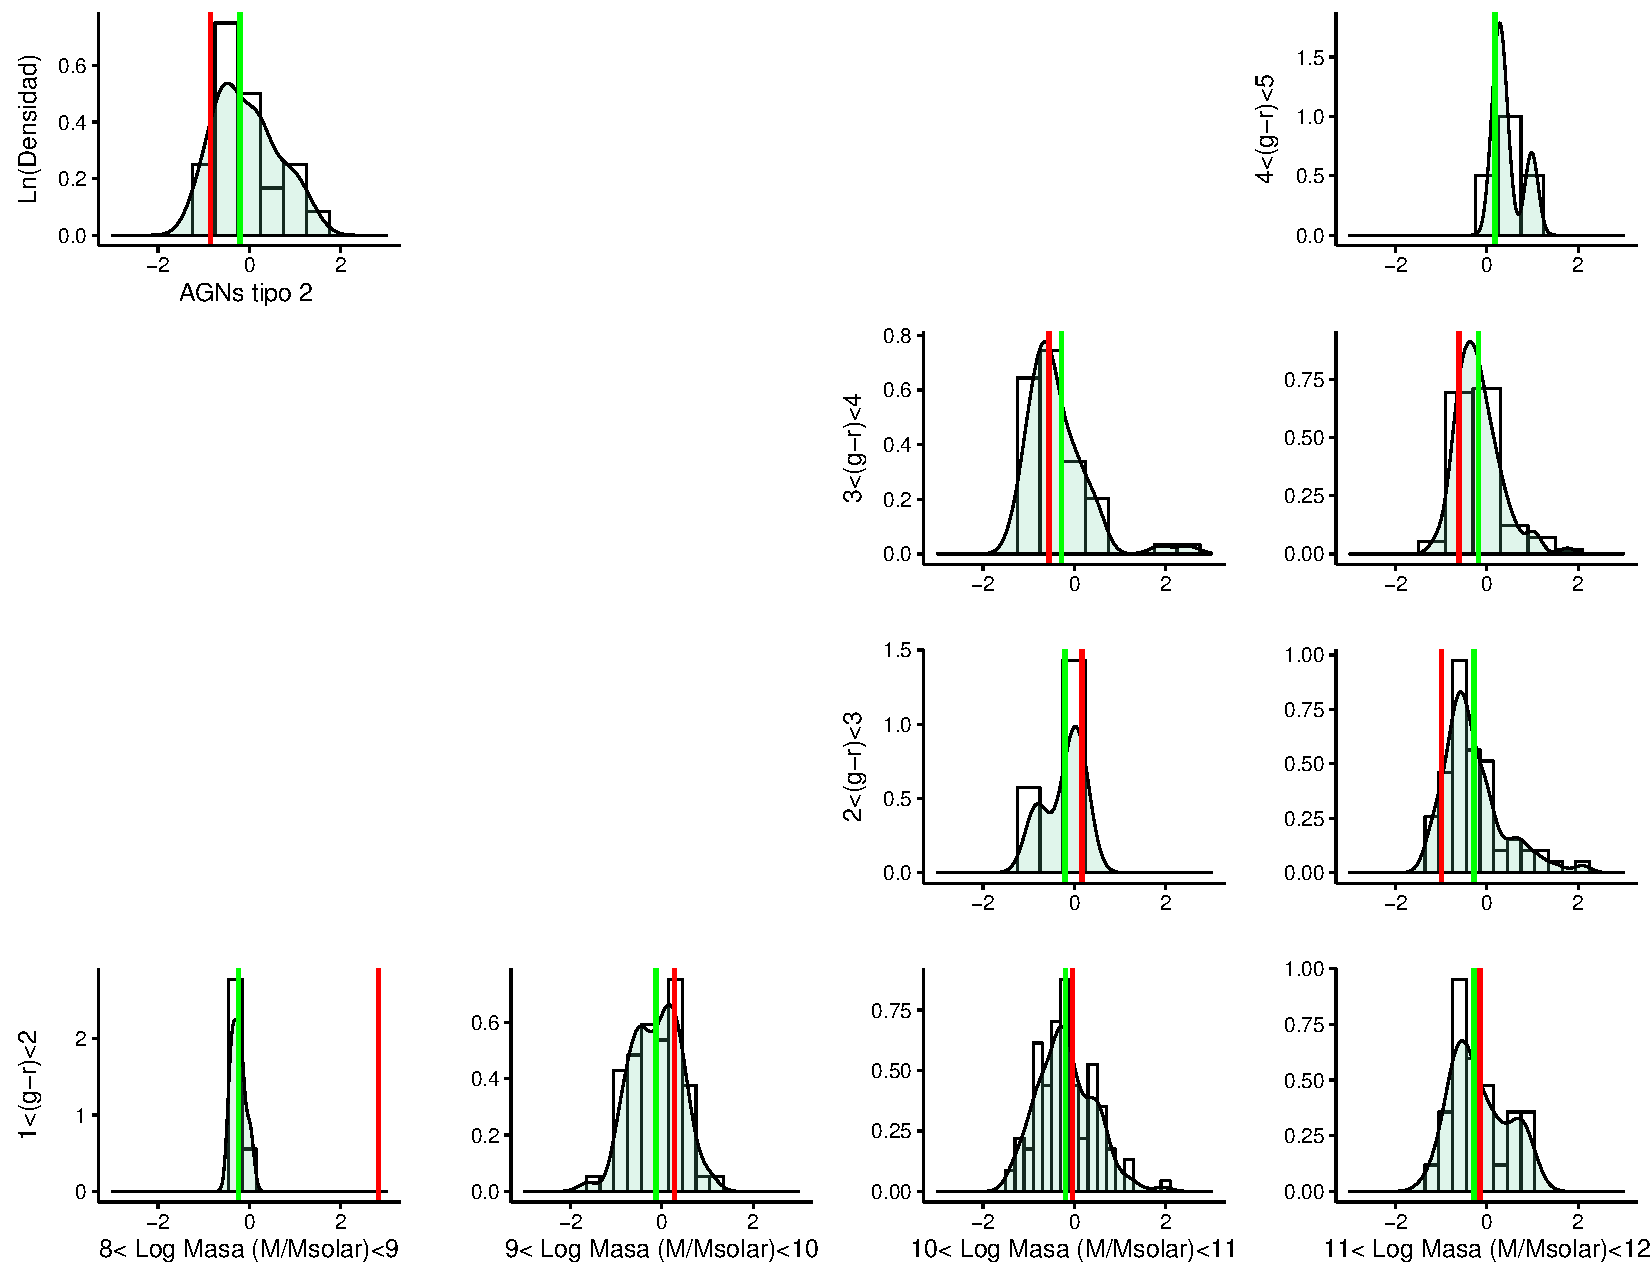
\includegraphics[scale=0.5]{log_chi_perl.pdf}
  \caption[Diagrama de distribuciones Log-Normal para $\chi^{2}_{\nu}$ en Color-Masa]{Diagrama Log-Normal para las distribuciones Color-Masa  de las $\chi^2_{\nu}$ pertenecientes a su intervalo correspondiente. La línea roja es la Log-Normal $\chi^2_{\nu}$ de UGC11680 para cada una de su categoría y la línea verde corresponde a la media Log-Normal de las distribuciones.En la esquina superior izquierda se colocaron las Log-Normal $\chi^2_{\nu}$ para los AGNs tipo 2  para referencia }
  \label{chi_todos_log}
\end{figure}



\subsection{Ajuste de $\chi^2_{UGC11680}$ con respecto a las Distribuciones Categóricas}


\noindent Como se mencionó anteriormente, la idea principal es buscar un ajuste de UGC11680 con respecto a cada $\chi^2_{\nu}$ de las categorías de la muestra tal que nos diga a que categoría se ``parece'' o ajusta mejor en su historia de formación estelar. Esto implicaría historias de formación estelar comunes  para las categorías que ajustan mejor con nuestra galaxia.  Observamos entonces que en la Figura \ref{chi_todos_mean} al ser $\chi^2_{\nu}$ una distribución no simétrica por construcción, el máximo no coincide necesariamente con la media de los datos. Además, la dispersión es un valor que oscila para cada categoría, por lo que para definir un ajuste que dependa de la media y su dispersión, consideramos que la distribución $\chi^2_{\nu}$ que construimos es una aproximación a la distribución Log-Normal, por lo que a todos los valores $\chi^{2}_{\nu}$  los escalamos tomando el logaritmo a cada uno de ellos. El resultado de esta distribuciones logarítmicas se muestran en la Figura \ref{chi_todos_log}, donde la $\chi^{2}_{\nu}$ de UGC11680  es la línea roja y la media la linea verde. Los rangos de las distribuciones son las mismos para todas las figuras. Debido a la transformación, obtenemos una distribución cuasi-Gaussiana para cada categoría y esto ya nos permitirá definir un ajuste con respecto a valores conocidos de una distribución normal. Teniendo en cuenta esto, para determinar a que categoría se asemeja más el mapa $SFH$ de UGC11680 comparamos ahora los valores de $\chi^{2}_{\nu}$ en escala logarítmica con respecto a la $\chi^2_{\nu}$ de UGC11680, normalizados a la dispersión logarítmica de los datos por categoría. Definimos entonces el ajuste de UGC11680 con respecto a estas como


\begin{equation}
AJ(\chi^2_{\nu})= \frac{ \ln(\chi^2_{UGC11680})  -  < ln (\chi^2_{cat})>} {\sigma_{\ln(\chi^2_{cat})}}
\end{equation}



\bigskip

\noindent Para obtener este valor de $AJ(\chi^2_{\nu})$ se iteró 3 veces con 2 lenguajes de programación diferentes (PERL y PYTHON)  para mejores resultados y estos se muestran en la tabla \ref{estadistica}

\begin{figure}[htbp]
\centering
\subfigure{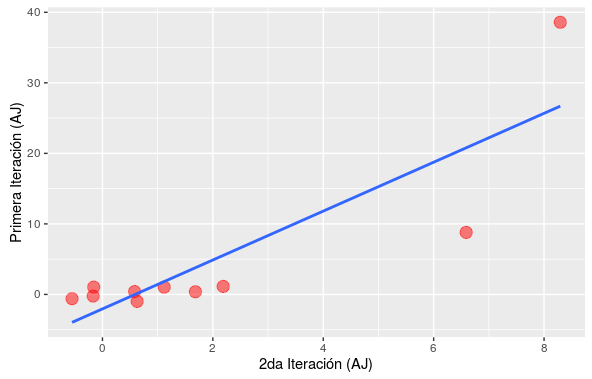
\includegraphics[width=70mm]{primer_scatter.png}}
\subfigure{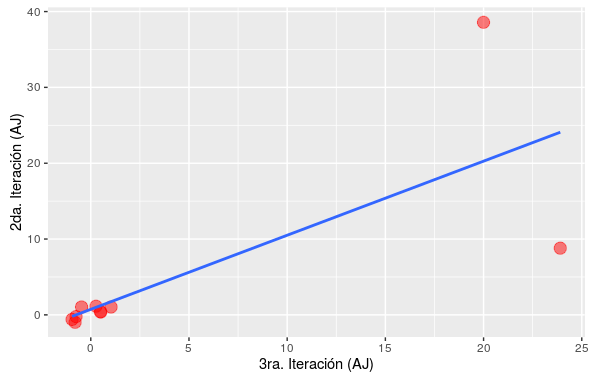
\includegraphics[width=70mm]{segundo_scatter.png}}
\caption[Correlación entre ajuster]{Correlación entre las diferentes iteraciones para calcular el valor de ajuste $|AJ(\chi^{2}_{\nu})|$ para la $\chi^{2}_{\nu}$ de UGC11680 con respecto a los promedios de cada categoría. Nótese que la dispersión para los valores mas grandes con respecto a la galaxia UGC11680 corresponden también a una $\chi^{2}_{\nu}$ grande, por lo que estos valores son de poca importancia estadística dentro del análisis.}
\label{correlacion}
\end{figure}


\begin{table}[!ht]
\centering
\begin{tabular}{||c | c | c | c ||}
\hline
\hline
Categoría & Primera Iteración &  2da. Iteración & 3era. Iteración \\
\hline
\hline
$(8<M_{\odot}<9)_{1<g-r<2}$  &  8.293 &  38.58 &  19.997 \\
$(9<M_{\odot}<10)_{1<g-r<2}$ &  1.118 & 1.035 &  1.032 \\
$(10<M_{\odot}<11)_{1<g-r<2}$ & 0.583 & 0.408 & 0.495 \\
$(10<M_{\odot}<11)_{2<g-r<3}$ & 1.684 &  0.378 & 0.508\\
$(10<M_{\odot}<11)_{3<g-r<4} $ & 0.167 & 0.226 &  0.749 \\
$(11<M_{\odot}<12)_{1<g-r<2} $ & 2.187 &  1.139 &  0.266 \\
$(11<M_{\odot}<12)_{2<g-r<3} $  & 0.628 &  0.986 & 0.798  \\
$(11<M_{\odot}<12)_{3<g-r<4} $  & 0.550 &  0.599 & 0.953 \\
$(11<M_{\odot}<12)_{4<g-r<5}$ & 6.589 & 8.792 &  23.90 \\
                        AGNs  & 0.158 & 1.037  & 0.469\\
\hline
\hline
\end{tabular}
\caption{Valores para el ajuste $AJ(\chi^2_{\nu})$ en tres diferentes iteraciones, utilizando mismo algoritmo pero en dos lenguajes de programación diferentes (PERL y PITHON). Nótese que la única discrepancia entre los diferentes ajustes corresponde a las categorías que contienen menos objetos. LA primera iteración corresponde a la reducción 1.5 de los datos de \textbf{CALIFA} y para los DR2 de los mismos. Las iteraciones 2 y 3 corresponden a la versión 2.2 de los datos, DR3, usando PERL PDL para la segunda  y PYTHON NumPy para la tercera. }
\label{estadistica}
\end{table}

\bigskip

\noindent Observando los valores de la tabla \ref{estadistica} aunque son del orden entre las diferentes categorías lo que se muestra en la figura \ref{correlacion} existe una cierta discrepancia entre los datos que se obtienen; esto se debe probablemente a la naturaleza de la definición para el ajuste $|AJ(\chi^{2}_{\nu})|$ así como la sensibilidad de los diferentes algoritmos en el truncamiento de valores cuando se define el logaritmo natural en diferentes lenguajes de programación. Obsérvese que los valores que más se dispersan en las Figuras en \ref{correlacion} corresponde a las categorías que contienen menos objetos y esto en sí mismo podría ser la causa de la dispersión. Sin embargo, esta discrepancia esta dentro del orden de los valores que se obtienen para cada ajuste, además de que la $\chi^{2}_{\nu}$ de UGC11680 esta muy alejada en realidad de la media de su distribución para las categorías con menos objetos, por lo que en si mismo, este ajuste no es tan significativo como los obtenidos para las otras categorías.


\bigskip

\noindent Técnicamente hablando, no podemos afirmar cual valor es el correcto para las iteraciones del ajuste de las $\chi^{2}_{\nu}$ de las historias de formación estelar, por lo que para obtener  el valor más cercano que nos indique el número más cercano para comparar  estas historia de formación de UGC11680 con respecto a sus diferentes categorías, usamos el valor medio de cada ajuste obtenido, generando así el que mejor se acerca a la $\chi^{2}_{\nu}$ de la historia de formación para la galaxia en cuestión. Estos valores se muestran para las distribuciones $\chi^{2}_{\nu}$ para cada categoría estudiada en la Tabla \ref{tab_LN2}. Los resultados se colocaron en orden descendente con respecto a $|AJ(\chi^2_{\nu})|$, de menor a mayor, donde el valor menor corresponde a un mejor ajuste de UGC11680 con respecto a la categoría indicada.



\bigskip

\begin{table}[!ht]
\centering
\begin{tabular}{||c | c | c | c | c||}
\hline
\hline
Categoría & $ \sigma_{\ln \chi^{2}_{\nu}}$ & $ <\ln(\chi^2_{cat})> $ & $\ln \chi^{2}_{UGC11680}$ & $|AJ(\chi^{2}_{\nu})|$ \\
\hline
\hline







$(10< \log M_{\odot}< 11)_{3<g-r<4}$  & 0.712  & -0.283  &-0.551  & 0.226 \\
                                  AGNs  & 0.540 & -0.205 & 0.445  & 0.469 \\
$(10< \log M_{\odot}< 11)_{1<g-r<2}$  & 0.608 & -0.192 & -0.035  & 0.495 \\
$(10< \log M_{\odot}< 12)_{2<g-r<3}$  & 0.596 & -0.205 & 0.058  & 0.508 \\
$(11< \log M_{\odot}< 12)_{3<g-r<4}$  & 0.501 & -0.181  & -0.612 & 0.599 \\
$(11<  \log M_{\odot}< 12)_{2<g-r<3}$ & 0.648 & -0.278  & -0.988  & 0.798 \\
$(9< \log M_{\odot}< 10)_{1<g-r<2}$   & 0.528 & -0.129 & 0.282  & 1.035 \\
$(11< \log M_{\odot}< 12)_{1<g-r<2}$  & 0.606 & -0.278 & -0.199  & 1.139 \\
$(11< \log  M_{\odot}< 12)_{4<g-r<5}$  & 0.503 & 0.183 & 11.55 & 8.792 \\
$(8< \log M_{\odot}< 9)_{1<g-r<2}$    & 0.157  & -0.237 & 2.83 & 19.997 \\



\hline
\hline
\end{tabular}
\caption{Tabla de los valores estadísticos para la comparación de UGC11680 con respecto a las categorías que se indican, comenzando con la dispersión, la media el valor $\chi^{2}_{\nu}$ de UGC11680 y finalmente el ajuste de su valor $\chi^{2}_{\nu}$ con respecto a cada una de ellas. El orden de los valores esta dado por $|AJ(\chi^{2}_{\nu})|$ del  menor a mayor que corresponderían al grado de mejor a menor ajuste de UGC11680 con respecto a las categorías indicadas. Todos los datos estadísticos se encuentran en escala logarítmica}
\label{tab_LN2}                              %etiqueta para referencia
\end{table}

\bigskip


\noindent Antes de interpretar los valores obtenidos, debemos recordar que estamos comparando historias de formación estelar por medio del mapa $SFH$, por lo que un parecido entre promedios por categorías y UGC11680 es un parecido en este contexto, de como los promedios de historia de formación estelar estudiadas  de la muestra de \textbf{CALIFA} y separadas por categorías coinciden con la galaxia espiral roja. De esta forma, con los valores de la tabla podemos Observamos el orden en que ajusto mejor la galaxia UGC11680:


\begin{itemize}

\item Ell mejor ajuste resulto ser para las galaxias rojas y masivas correspondientes a la categoría a la que pertenece UGC11680 $\sim 10^{10} \log M_{\odot}$ , $3<\text{color}<4$, esto nos indicaría que UGC11680 ajusta en su historia de formación estelar con las de su categoría.


\item  El segundo mejor ajuste corresponde a el grupo de los AGNs. Esto nos indicaría que el AGN de alguna forma influye o altera la formación estelar, al menos para las galaxias de la muestra.

\item  El tercer y cuarto mejor ajuste corresponde al grupo de  de galaxias  de masa intermedia, que se encuentran en el valle verde ($10< \log M_{\odot} < 11$ color $1<g-r<2$) y ($10< \log M_{\odot}< 11$ color $2<g-r<3$). Este resultado es interesante ya que la galaxia aun siendo de color rojo en el óptico, coincide en formación estelar con las galaxias en la llamada zona de transición.

\item Por último, los últimos mejores ajustes corresponden a las galaxias más masivas y rojas masivas  comenzando por las mas rojas ($10< \log M_{\odot}< 11)$ color $3<g-r<4$) seguidas por las menos rojas que las anteriores ($11< \log M_{\odot}< 12$ color $2<g-r<3$).


\end{itemize}

\bigskip


\noindent Los demás valores del ajuste corresponden a las galaxias que menos encajan con UGC11680, que en general son las galaxias que están en la nube azul, ya sean masivas o no, así como las galaxias mas masivas y rojas de toda la muestra, que aunque contiene pocos objetos, la discrepancia es demasiada como para ser estadísticamente relevante. Podríamos decir que el ajuste en historia de formación estelar  de UGC11680 coincide con las de su categoría, las galaxias de masa intermedia en el rango del color rojo, los AGNs tipo 2, las galaxias de masa intermedia en la zona de transición conocida como el valle verde y finalmente a las galaxias masivas en los límites entre la secuencia roja y la zona de transición. Los demás ajustes se alejan de un valor relevante para el estudio de la galaxia por lo que su valor no nos indican alguna semejanza en historia de formación estelar para que pueda considerarse como un ``parecido'' dentro de la definición que hemos estado manejando. Estos resultados ya nos indican que UGC11680 es una galaxias peculiar, en donde el AGN y su masa juegan un papel importante y que fueron determinantes para detener la formación estelar desde dentro hacia afuera, empezando a épocas cosmológicas tempranas ($\sim$ 9 Gyrs).









   % ~20 páginas - Presentar los resultados tal cual son, y analizarlos.
\chapter{Conclusiones}


\lettrine[lines=1]{B}asados en los resultados en las secciones anteriores, podemos describir la historia de formación estelar de UGC11680 como sigue: los primeros resultados, el mapa $SFH$ de la Figura \ref{sfh_ugc11680} nos muestran un apagado de formación estelar en las zonas centrales  de esta galaxia ya que el gradiente temporal de su densidad de masa superficial tiene un cambio abrupto a edades tempranas, en forma de corte, y conforme se avanza a edades cosmológicas  actuales este corte corre diagonalmente, lo que implica un apagado en formación a radios más grandes y por lo tanto a zonas más externas.

\bigskip

\noindent El perfil de densidad de masa radial a diferentes tiempos de la Figura \ref{perfil_radial} nos indica que en efecto, el apagado es interno (cambio en gradientes), comparado con promedios de diferentes tipos de galaxias. El ensamblaje de masa además se comporta en UGC11680 con lo encontrado en trabajos anteriores \citep{perez2013} y como se muestra en la Figura \ref{ensamblaje_log}. Por lo tanto, la galaxia acumuló masa de dentro hacia afuera y el apagado comienza internamente, lo que también se muestra en su tasa de formación estelar temporal.

\bigskip

\noindent En todos los casos, el registro fósil señala crecimiento dentro-fuera y apagado de la misma forma, además de gradientes radiales que señalan que las partes internas tienen procesos que detienen este proceso de acumulación de masa estelar. Los promedios en cambio, muestran ensamblajes encontrados en otros trabajos \cite{perez2013} ({\color{red} Ibarra-Medel, et.al. (Submitted) }).

\bigskip

\noindent Los promedios de la Figura \ref{CMD} muestran también que la masa es una variable fundamental en el proceso de acumulación de masa temporal ya que los mapas  $SFH$ promediados por color-masa muestran una tendencia de formación estelar: entre más masivas , más rápido ensamblan estrellas  lo que no se muestra en las galaxias menos masivas y azules: estas siguen formando estrellas, según su $SFH$ promediado.

\bigskip


\noindent Entonces ¿De que forma encaja la historia de ensamblaje de masa de UGC11680 con respecto a las demás galaxias de la muestra? Todo parece indicar con las distribuciones de la Figura \ref{chi_todos_mean} y los resultados de la tabla \ref{tab_LN2} que UGC11680 encaja con las galaxias  rojas y de masa intermedia (las galaxias con masa  $\sim 10^{10} M_{\odot}$, con colores entre $3<g-r<4$ ), con el grupo de AGNs, las galaxias de masa intermedia en el valle verde  ($\sim 10^{10} M_{\odot}$, con colores entre $1<g-r<2$ y $2<g-r<3$ ) y  las galaxias masivas en el valle verde ($\sim 10^{11} M_{\odot}$ colores entre $2<g-r<3$) . 


\bigskip

\noindent Estos resultados son interesantes ya que entonces tenemos evidencia espacialmente resuelta de que UGC11680, siendo una galaxia espiral roja, ensambló su masa de dentro hacia afuera, con un apagado abrupto de la misma forma y que su historia de formación estelar es parecida o coincide mejor con galaxias de su masa y color, pero tambien con galaxias con AGN asi como las que se encuentran en el valle verde. 
\bigskip


\noindent También es interesante notar que el ajuste de la sección de comparación por medio de la distribución $\chi^{2}_{\nu}$ la masa parece ser un factor importante para que UGC11680 ensamblara y apagara su formación estelar rapidamente, ya que comienza con un ajuste con las galaxias de masa intermedia, seguidas de las galaxias más masivas, lo que nos indica que la masa es determinante en la formación y posterior ensamblaje de UGC11680, algo encontrado en trabajos anteriores para galaxias de la muestra de \textbf{CALIFA} \citep{perez2013}. 

\bigskip

\noindent Esto claro, no implica que sólo el AGN haya contribuido para el apagado de la formación estelar de UGC11680, sino que pudo iniciarlo para que procesos seculares como alguna interacción no violenta ó algún otro proceso físico haya continuado con el proceso, debido a que la galaxia siguió formando estrellas, pero a una tasa baja, lo que la colocó debajo de las galaxias SF pero sobre las galaxias retiradas  de la Figura \ref{sfr_califa}. 

\bigskip

\noindent Finalmente, por el análisis en la sección de poblaciones estelares, podemos excluir el polvo como causante de su color UGC11680:  entonces, debido al apagado rápido en formación estelar desde dentro hacia afuera, la galaxia pasó por el valle verde y  se situó en su posición dentro de la secuencia roja sólo por formación estelar promedio que mide el diagrama color-magnitud. Esto nos indica que UGC11680 es una galaxia peculiar con un ensamblaje de masa de dentro hacia afuera y que su color en el óptico resulta de una combinación de procesos internos de apagado abrupto en las zonas centrales, aunque sus poblaciones espacialmente resueltas indican que este apagado no fue total, sino de alguna forma regulado desde dentro hacia afuera, ya que la galaxia continua formando estrellas aunque a  una tasa baja a diferentes épocas cosmológicas en su historia de formación estelar. 




            % ~5 páginas - Resumir lo que se hizo y lo que no y comentar trabajos futuros sobre el tema

%%%%%%%%%%%%%%%%%%%%%%%%%%%%%%%%%%%%%%%%%%%%%%%%%%%%%
%                   APÉNDICES                       %
%%%%%%%%%%%%%%%%%%%%%%%%%%%%%%%%%%%%%%%%%%%%%%%%%%%%%
\appendix
% this file is called up by thesis.tex
% content in this file will be fed into the main document
\chapter{Regiones Ionizadas}



\lettrine[lines=1]{A}unque es un trabajo sobre poblaciones estelares, es interesante saber por que consideramos a UGC11680 como una galaxia espiral con un AGN  tipo 2. Este tipo de análisis se puede realizar ya sea con cada espectro de las galaxias de la muestra o espectros integrados para resultados estadísticos. Este proceso se  hace con las líneas de emisión de cada espectro de la galaxia, lo cual hacemos un breve resumen del análisis realizado, para ver que es así.


\begin{figure}[!ht]
  \centering
  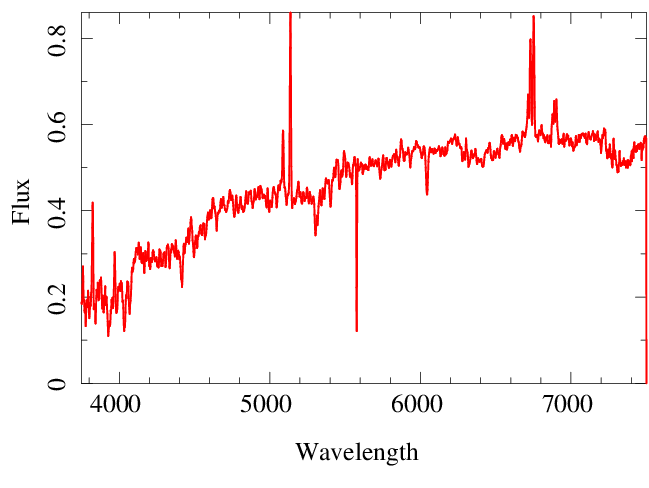
\includegraphics[width=4in]{spec_cen_UGC11680NED01.png}
  \caption[Espectro central UGC11680]
   {Espectro en el óptico de la region central de UGC11680 sacado directamente de su cubo de datos, en \textbf{CALIFA}. Las longitudes de onda están en sus valores en el marco de referencia del laboratorio. Notese la ausencia de componentes de líneas anchas y las líneas prohibidas del oxígeno ([O III] $\lambda \lambda$4959, 5007 \text{\AA}, [O I] $\lambda$6300 \text{\AA}), y las líneas de  nitrógeno ([N II]  $\lambda \lambda$ 6548, 6583 \text{\AA}), y silicon ([S II] $\lambda \lambda$6716, 6731 \text{\AA}), características de un AGN tipo II.  Nótese que la linea de  [N II] esta casi mezclada con  $H_{\alpha}$ en $\lambda$ = 6563 \text{\AA} }
\label{espectro}
\end{figure}


\begin{figure}[!ht]
  \centering
  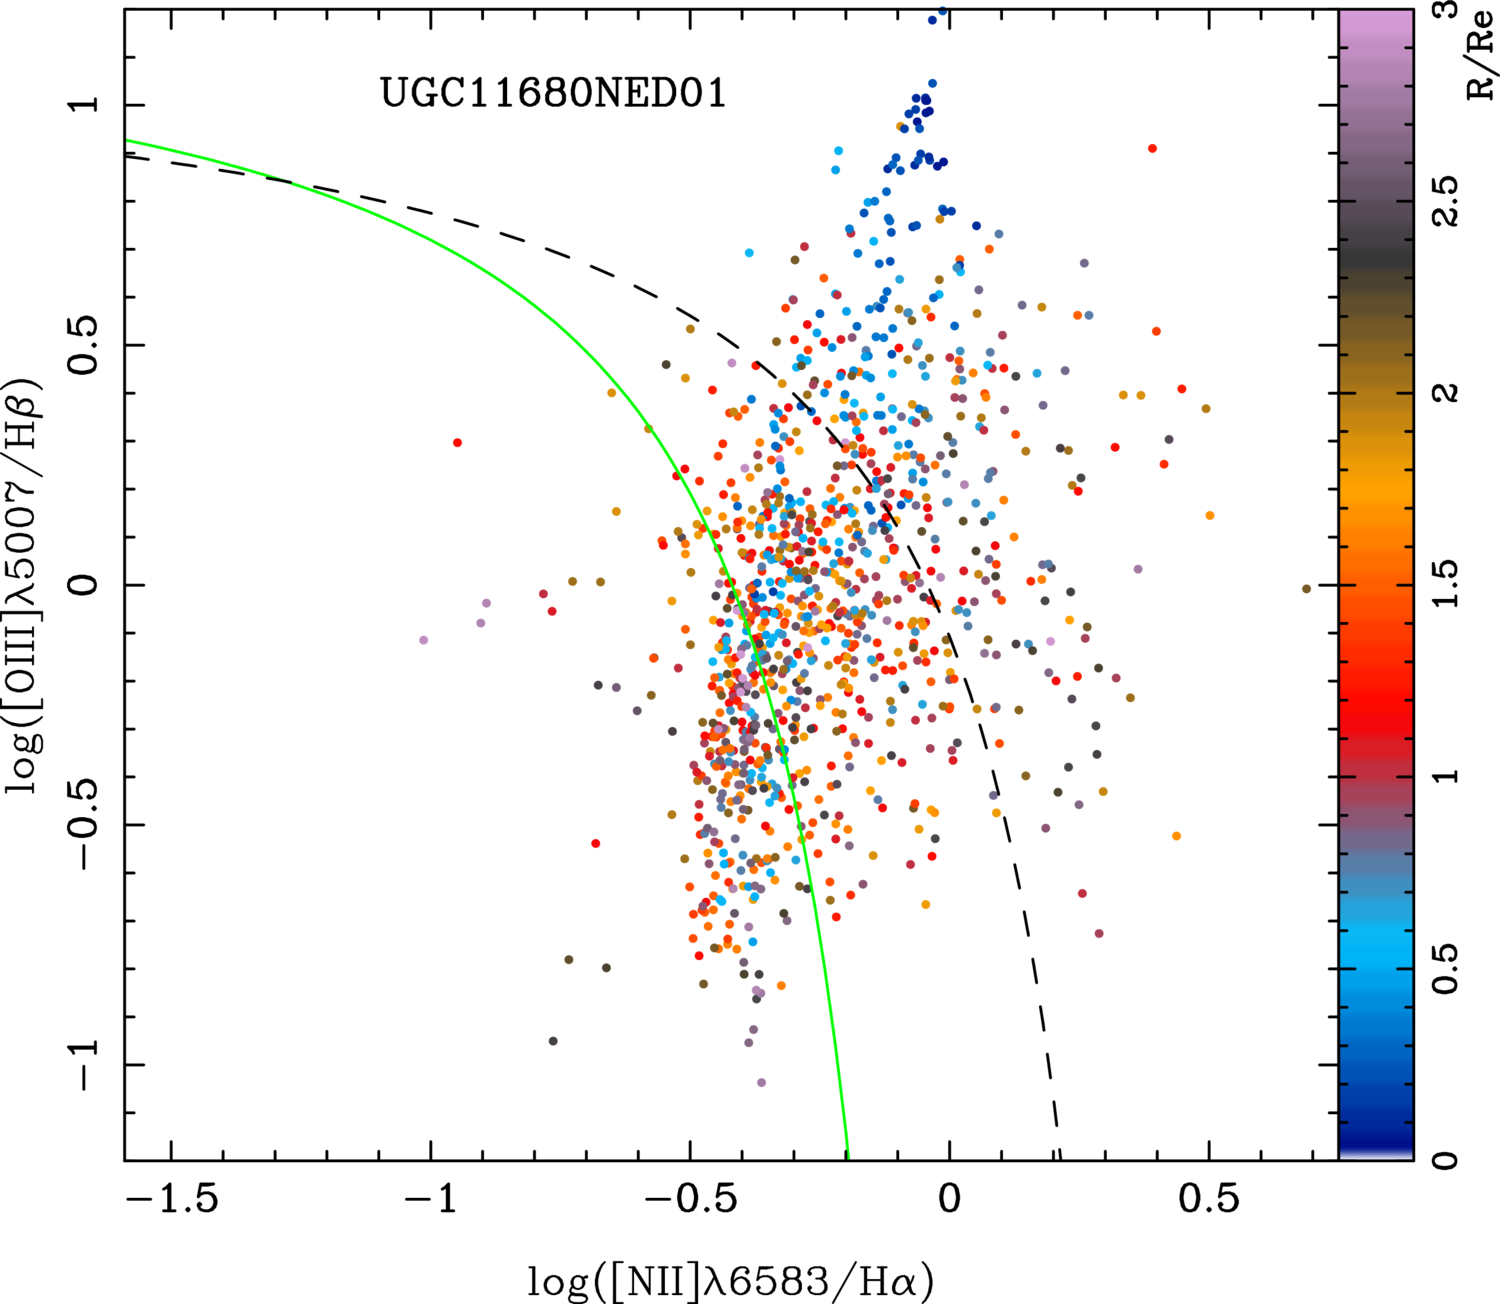
\includegraphics[scale=0.2]{1UGC11680NED01_proc_elines4.png}
  \caption[ Diagrama bpt UGC11680]
   {Diagrama BPT de  UGC11680,usando las líneas ya corregidas de [O III]$\lambda$5007/$H_{\beta}$ vs.
[N II]$\lambda$6583/$H_{\alpha}$. Los puntos azules indican zonas galactrocentricas amarillas a rojas la zona media y moradas las afueras. La line solida representa un modelo de region HII la linea punteada, conocida como la línea de ``Kewley'' divide la ionización por AGN de las zonas ionizadas por regiones HII, mientras que la linea verde denota la linea de  ``Kauffmann''. Obsérvese que a pesar de la ionización del AGN, UGC11680 sigue mostrando regiones HII y por lo tanto formación estelar en sus afueras. }
\label{bpt}
\end{figure}


\section{Diagramas BPT}

\bigskip

Tras el descubrimiento de galaxias espirales con un núcleo muy brillante que emite
(líneas de emisión de varios miles de km/s) (\citet{seyfert1941}),
se hizo evidente que estos núcleos galácticos eran el lugar de una violenta,
actividad no estelar (\citet{burbidge1963}), tal vez de la misma naturaleza que se encontró en los cuásares.
Heckman  realizó un análisis espectroscópico de los núcleos de una muestra completa
de 90 galaxias, y  encontró que la presencia de baja ionización nuclear (LINERS) eran bastante comunes, y parecían ser
la versión reducida de los núcleos Seyfert. \cite{baldwin1981} fueron los
primero en proponer diagnósticos espectroscópicos sobre la base de relaciones de línea de emisión
para distinguir galaxias normales  de formación estelar de los AGNs. El más famoso es el que compara los cocientes de líneas
[O III] $\lambda$5007/$H_{\beta}$ vs [N II]$\lambda$6583/$H_{\alpha}$ a menudo referido como el diagrama de BPT (por Baldwin, Phillips,
Y Terlevich).

\bigskip

\noindent \citet{osterbrock1987} propusieron diagramas adicionales: [O III] $\lambda$5007/$H_{\beta}$ vs
[S II] $\lambda$6725 /$H_{\alpha}$, y [O III] $\lambda$5007/$H_{\beta}$ vs [S i] $\lambda$6300/$H_{\alpha}$.
Como es conocido \citet{osterbrock1989}, las regiones H II  forman una
secuencia mas estrecha en estos diagramas. Sólo unos años después, \citet{kewley2001}  construyeron un \textsl{grid} de
modelos de fotoionización a fin de determinar un límite superior teórico
a la ionización por las estrellas masivas en el diagrama de BPT. Este límite superior,
más adelante se hace referencia como la ``línea de Kewley". \citet{kauffmann2003} desplazaron esta línea a la izquierda para definir un límite empírica entre galaxias normales de formación de estrellas y que tienen un AGN (la línea de ``Kauffmann")

\bigskip

\noindent De esta forma,Como tenemos un ejemplo típico de una galaxia  con resolución espacial, podemos hacer un diagrama BPT sólo para una galaxia y por lo tanto cada punto representa un zona en nuestra galaxia. La figura \ref{bpt} representa
la gráfica de [O III] $\lambda$5007/$H_{\beta}$ vs [N II]$\lambda$6584/$H_{\alpha}$ de un diagrama BPT para UGC11680.
En este gráfico podemos ver dos líneas curvas diferentes. Los puntos por encima y a la derecha de la línea de puntos representa
zonas ionizadas por el AGN, mientras que los puntos de abajo y hacia la izquierda para
la línea de trazos representan zonas de formación de estrellas. Los
puntos en el medio representan zonas que tienen características
de ambas regiones ionizadas por AGN  y de formación de estrellas HII. Observamos entonces que para UGC11680 las regiones centrales, se encuentran ionizadas por procesos no estelares, lo que puede ser la presencia de un AGN. Obsérvese también que esta galaxia tiene presencia de regiones HII en las afueras, lo que implica que esta galaxia sigue formando estrellas.

\bigskip

\noindent Resumiendo, el espectro de la zona central, así como su diagrama BPT, nos indican que UGC11680 es una galaxia con AGN tipo II, y que a pesar de no ser notorio en sus imágenes en el óptico, esta galaxia sigue formando estrellas aunque a una tasa baja, debido a la presencia de regiones HII en las zonas exteriores dadas por el radio efectivo. Este resultado,coincide con los resultados que se obtuvieron por análisis de poblaciones estelares, es decir, aunque la galaxia tiene un color rojo en el óptico, esta sigue formando estrellas, aunque a una tasa baja.

\chapter{Tabla de conversión}

\begin{table}[!ht]
\centering
\begin{tabular}{||c | c | c||}
\hline
\hline
Look back in time (Gyrs) & Edad (Gyrs) & $\sim$ redshift $z$ \\
\hline
\hline


1.122  & 13.0  & 0.070  \\
1.259 & 12.8 & 0.080   \\
1.42  & 12.2 & 0.083  \\
2.0  & 11.8 & 0.15  \\
2.5 & 11.4 & 0.19  \\
3.55  & 10.6 & 0.3  \\
4.5  & 9.4 & 0.4  \\
6.3 & 8.4 & 0.65  \\
8.0   &  6.2 & 0.8  \\
10.0  & 4.1  & 1.7  \\
12.6  & 1.5  & 4.7  \\
14.2  & 0.1  & 19  \\

\hline
\hline
\end{tabular}
\caption{Tabla de conversión entre edades para el estudio de la historia de formación estelar usada en la tesis asi como su aproximación en redshift $z$, usando los datos cosmologicos $\Omega_m = 0.317$ , $\Omega_{\Lambda}=0.683$ y $H_0 = 67.15$ km/s/Mpc \citep{plank2014}} 
\label{tab_conversion}                              %etiqueta para referencia
\end{table}
               % Colocar los circuitos, manuales, código fuente, pruebas de teoremas, etc.

%%%%%%%%%%%%%%%%%%%%%%%%%%%%%%%%%%%%%%%%%%%%%%%%%%%%%
%                   REFERENCIAS                     %
%%%%%%%%%%%%%%%%%%%%%%%%%%%%%%%%%%%%%%%%%%%%%%%%%%%%%
% existen varios estilos de bilbiografía, pueden cambiarlos a placer
\bibliographystyle{apj} % otros estilos pueden ser abbrv, acm, alpha, apalike, ieeetr, plain, siam, unsrt

%El formato trae otros estilos, o pueden agregar uno que les guste:
%\bibliographystyle{Latex/Classes/PhDbiblio-case} % title forced lower case
%\bibliographystyle{Latex/Classes/PhDbiblio-bold} % title as in bibtex but bold
%\bibliographystyle{Latex/Classes/PhDbiblio-url} % bold + www link if provided
%\bibliographystyle{Latex/Classes/jmb} % calls style file jmb.bst

\bibliography{Bibliografia/referencias}             % Archivo .bib


\end{document}
